\documentclass[12pt,a4paper]{article}

\usepackage[utf8]{inputenc}
\usepackage[T1]{fontenc}
\usepackage{lmodern}
\usepackage[ngerman]{babel}
% German support via inputenc only
% microtype removed for compatibility
\usepackage{geometry}
\geometry{a4paper, margin=2.5cm}

\usepackage{amsmath, amssymb, amsthm, mathtools}
\usepackage{thmtools}
\usepackage{graphicx}
\usepackage{float}
\usepackage{caption}
\usepackage{subcaption}
\usepackage{booktabs}
\usepackage{array}
\usepackage{longtable}
\usepackage{xcolor}
\usepackage{hyperref}
\usepackage{tikz}
\usetikzlibrary{shapes.geometric, arrows.meta, positioning, calc, fit, matrix, decorations.pathreplacing, backgrounds}
\usepackage{pgfplots}
\pgfplotsset{compat=1.18}
\usepackage{algorithm}
\usepackage{algpseudocode}
\usepackage{enumitem}
\usepackage{cleveref}
\crefname{section}{Kapitel}{Kapitel}
\Crefname{section}{Kapitel}{Kapitel}
\crefname{subsection}{Abschnitt}{Abschnitte}
\Crefname{subsection}{Abschnitt}{Abschnitte}
\usepackage{setspace}
\usepackage{fancyhdr}
\usepackage{titlesec}
\usepackage{abstract}

\setlist[itemize,1]{label=--}

% bibliography packages

% ── Farben ────────────────────────────────────────────────────────────────────
% Kopfzeilenhöhe für fancyhdr
\setlength{\headheight}{13.6pt}
\definecolor{darkblue}{RGB}{0,51,102}
\definecolor{midblue}{RGB}{31,119,180}
\definecolor{teal}{RGB}{42,157,143}
\definecolor{crimson}{RGB}{220,50,47}
\definecolor{amber}{RGB}{244,162,97}
\definecolor{lightgray}{RGB}{245,245,245}
\definecolor{codelgray}{RGB}{250,250,250}

% ── Hyperref ──────────────────────────────────────────────────────────────────
\hypersetup{
  colorlinks=true,
  linkcolor=darkblue,
  citecolor=teal,
  urlcolor=midblue,
  pdftitle={Graphenstrukturelles Denken als universelles kognitives Paradigma},
  pdfauthor={Stephan Epp},
  pdfsubject={Kognitive Graphentheorie, Neuronale Netze, Strukturdenken}
}

% ── Theorem-Umgebungen ────────────────────────────────────────────────────────
\theoremstyle{plain}
\newtheorem{theorem}{Theorem}[section]
\newtheorem{lemma}[theorem]{Lemma}
\newtheorem{korollar}[theorem]{Korollar}
\newtheorem{proposition}[theorem]{Proposition}

\theoremstyle{definition}
\newtheorem{definition}[theorem]{Definition}
\newtheorem{axiom}[theorem]{Axiom}
\newtheorem{beispiel}[theorem]{Beispiel}

\theoremstyle{remark}
\newtheorem{bemerkung}[theorem]{Bemerkung}
\newtheorem{notation}[theorem]{Notation}

\renewcommand{\proofname}{Beweis}

% ── Abkürzungen ───────────────────────────────────────────────────────────────
\setlength{\emergencystretch}{2em}
\newcommand{\GG}{\mathcal{G}}
\newcommand{\VV}{\mathcal{V}}
\newcommand{\EE}{\mathcal{E}}
\newcommand{\cNN}{\mathcal{N}}
\newcommand{\NNs}{\mathbb{N}}
\newcommand{\HH}{\mathcal{H}}
\newcommand{\RR}{\mathbb{R}}
\newcommand{\ZZ}{\mathbb{Z}}
\newcommand{\NNnull}{\mathbb{N}_0}
\newcommand{\KNN}{\text{KNN}}
\newcommand{\MLP}{\text{MLP}}
\newcommand{\SA}{\textnormal{\textsc{Subgraph Algorithmus}}}
\newcommand{\norm}[1]{\left\|#1\right\|}
\newcommand{\inner}[2]{\langle #1,\, #2 \rangle}



\title{\textbf{Graphenstrukturelles Denken als universelles kognitives Paradigma} \\ 
	\Large Formale Grundlagen, Isomorphiebeweise und strukturelle Harmonie mit Neuronalen Netzen}
\author{Stephan Epp}
\date{31. März 2026}

% ─────────────────────────────────────────────────────────────────────────────
\begin{document}

\maketitle
\tableofcontents
\newpage

% =============================================================================
\section{Einleitung}
\label{sec:einleitung}
% =============================================================================

Diese Arbeit stellt eine formale Theorie des \emph{graphenstrukturellen Denkens} auf und beweist dessen strukturelle Isomorphie zu den Berechnungsmodellen moderner neuronaler Netze und großer Sprachmodelle (LLMs). Wir zeigen, dass das menschliche Gehirn, künstliche neuronale Netze, Transformer-Architekturen und abstrakte kognitive Prozesse dieselbe fundamentale mathematische Struktur teilen: gerichtete, gewichtete Graphen mit hierarchischer Schichtung. Diese strukturelle Konvergenz erklärt, warum graphenorientierte Denker eine außergewöhnliche Synergie mit KI-basierten Werkzeugen entwickeln. Wir formalisieren den Begriff des \emph{kognitiven Graphen}, führen Graph-Isomorphie als Harmoniemaß ein und beweisen mehrere Kerntheoreme über Strukturerhalt, Aufmerksamkeitsgraphen und hierarchische Subgrapheinbettungen. Der \SA{} (Epp~2026) dient dabei als durchgehendes Leitbeispiel einer praktischen Realisierung dieses Paradigmas. Abschließend werden Implikationen für Mensch-KI-Kollaboration, epistemische Modellierung und kognitive Informatik diskutiert.

\subsection{Motivation und Problemstellung}

Warum harmonieren manche Menschen intuitiv mit künstlicher Intelligenz, während andere einen erheblichen Reibungswiderstand im Umgang mit KI-basierten Werkzeugen verspüren? Diese Frage ist nicht trivial und lässt sich nicht allein durch Faktoren wie technisches Vorwissen, Bildungsgrad oder Kreativität erklären. Die vorliegende Arbeit vertritt die These, dass die entscheidende Variable eine \emph{fundamentale kognitive Struktur} ist: das graphenstrukturelle Denken.

Erst diese Denkweise erlaubt und ermöglicht die Sicht auf das Leben, wie es wirklich zu sehen ist. Eine andere Denkweise tut das nicht. Viele Beispiele bestätigen diese Aussage. Es ist ein Beweis durch Widerspruch zu führen, dass nur diese Denkweise dazu geeignet ist. Angenommen, es gibt eine andere Denkweise, die nicht dieser Denkweise entspricht, dann muss diese andere Denkweise entweder eine andere Struktur haben oder gar keine Struktur. Wenn sie gar keine Struktur hat, ist sie nicht greifbar und nicht wirklich anwendbar. Wenn sie eine andere Struktur hat, ist zu untersuchen, wie diese Struktur aussieht. Was ist eine Struktur? Wie kann die Denkweise anders als durch Graphen strukturell beschrieben werden? Was liegt dem Denken zugrunde? Das Gehirn des Menschen. Das Einzige, was wir strukturell beschreiben können von der Materie her, ist das Gehirn. Was wir nicht beschreiben können, ist der Geist des Menschen. Es lohnt sich also hier nur die Betrachtung des Gehirns in seiner Struktur. Betrachtet man aber die Struktur des Gehirns, fällt sofort auf, dass die beste Struktur gegeben ist durch Graphen.

Unter graphenstrukturellem Denken verstehen wir die natürliche Disposition eines kognitiven Systems, Wissen, Konzepte und Probleme primär als \emph{Knoten und Kanten in einem relationalen Netzwerk} zu repräsentieren, anstatt als lineare Sequenzen oder hierarchisch-baumartige Taxonomien. Ein Mensch mit dieser Disposition denkt in Verbindungen, Pfaden, Zyklen, Teilgraphen und Isomorphien -- nicht in Listen.

Moderne neuronale Netze, insbesondere Transformer-basierte Sprachmodelle, realisieren exakt dieselbe mathematische Struktur auf algorithmischer Ebene. Die \emph{Self-Attention}-Schicht eines Transformers berechnet für jede Eingabe einen vollständigen gewichteten Graphen über alle Tokens. Das Forward-Pass durch ein mehrschichtiges Netz ist ein gerichteter azyklischer Graph (DAG) von Tensoroperationen. Die Gewichtsmatrizen kodieren Kantengewichte in einem hochdimensionalen Vektorraum.

Diese strukturelle Kongruenz ist keine Metapher -- sie ist mathematisch präzise fassbar und formal beweisbar. Die vorliegende Arbeit liefert diesen formalen Nachweis.

\subsection{Überblick und Beiträge}

Die Kernbeiträge dieser Arbeit sind:

\begin{enumerate}[label=\textbf{(B\arabic*)}]
  \item \textbf{Formale Definition des kognitiven Graphen:} Wir führen den Begriff $\GG_{\text{kog}}$ als mathematisches Objekt ein und zeigen seine strukturellen Eigenschaften (\cref{sec:kognitivergraph}).

  \item \textbf{Graphenmodell neuronaler Netze:} Wir formalisieren sowohl biologische als auch künstliche neuronale Netze als spezielle Klassen gewichteter Digraphen und beweisen deren Struktureigenschaften (\cref{sec:knn}).

  \item \textbf{Isomorphiesätze:} Wir beweisen mehrere Theoreme über die strukturelle Isomorphie zwischen kognitiven Graphen, neuronalen Netzen und Transformer-Attention-Graphen (\cref{sec:isomorphie}).

  \item \textbf{Hierarchische Graph-Einbettung:} Wir formalisieren Graph-of-Graphs-Struk\-turen und beweisen Erhaltungssätze für Subgraph-Einbettungen (\cref{sec:hierarchie}).

  \item \textbf{Harmoniekoeffizient:} Wir definieren ein quantitatives Maß $\kappa(\GG_1, \GG_2)$ für die strukturelle Harmonie zweier kognitiver Systeme (\cref{sec:harmonie}).

  \item \textbf{Anwendung: Subgraph Algorithmus:} Wir analysieren den \SA{} (Epp~2026) als praktische Instanz des graphenstrukturellen Denkparadigmas (\cref{sec:subgraph}).
\end{enumerate}

\subsection{Struktur der Arbeit}

\Cref{sec:grundlagen} legt die mathematischen Grundlagen der Graphentheorie fest. \Cref{sec:kognitivergraph} definiert den kognitiven Graphen. \Cref{sec:knn} formalisiert neuronale Netze als Graphen. \Cref{sec:isomorphie} beweist die zentralen Isomorphiesätze. \Cref{sec:hierarchie} behandelt Graph-Hierarchien. \Cref{sec:harmonie} führt den Harmoniekoeffizienten ein. \Cref{sec:subgraph} analysiert den Subgraph Algorithmus. \Cref{sec:impl} diskutiert Implikationen. \Cref{sec:diskussion} beleuchtet verwandte Arbeiten und Grenzen der Theorie. \Cref{sec:schluss} fasst die zentralen Ergebnisse zusammen und entwickelt einen umfassenden Ausblick auf zukünftige Forschungsrichtungen.

% =============================================================================
\section{Mathematische Grundlagen der Graphentheorie}
\label{sec:grundlagen}
% =============================================================================

\subsection{Grundlegende Definitionen}

\begin{definition}[Gerichteter gewichteter Graph]
\label{def:graph}
Ein \emph{gerichteter gewichteter Graph} ist ein Tupel
\[
  \GG = (V,\, E,\, w)
\]
wobei:
\begin{itemize}
  \item $V = \{v_1, v_2, \ldots, v_n\}$ die endliche Menge der \emph{Knoten} (Vertices) ist,
  \item $E \subseteq V \times V$ die Menge der \emph{gerichteten Kanten} (Edges) ist,
  \item $w : E \to \RR$ eine \emph{Gewichtsfunktion} ist.
\end{itemize}
Wir bezeichnen $|V| = n$ als die \emph{Ordnung} und $|E| = m$ als die \emph{Größe} von $\GG$.
\end{definition}

\begin{definition}[Adjazenzmatrix]
\label{def:adjazenz}
Die \emph{gewichtete Adjazenzmatrix} $A \in \RR^{n \times n}$ eines Graphen $\GG = (V, E, w)$ ist definiert durch:
\[
  A_{ij} = \begin{cases} w(v_i, v_j) & \text{falls } (v_i, v_j) \in E \\ 0 & \text{sonst.} \end{cases}
\]
\end{definition}

\begin{definition}[Subgraph]
\label{def:subgraph}
Ein Graph $\GG' = (V', E', w')$ heißt \emph{Subgraph} von $\GG = (V, E, w)$, geschrieben $\GG' \subseteq \GG$, falls $V' \subseteq V$, $E' \subseteq E \cap (V' \times V')$ und $w' = w|_{E'}$.
\end{definition}

\begin{definition}[Graphisomorphismus]
\label{def:isomorphismus}
Zwei Graphen $\GG_1 = (V_1, E_1, w_1)$ und $\GG_2$ mit $\GG_2 = (V_2, E_2, w_2)$ heißen \emph{isomorph}, geschrieben $\GG_1 \cong \GG_2$, falls eine bijektive Abbildung $\phi: V_1 \to V_2$ existiert, sodass:
\[
  (u,v) \in E_1 \iff (\phi(u), \phi(v)) \in E_2
  \quad \text{und} \quad
  w_1(u,v) = w_2(\phi(u), \phi(v)) \quad \forall\, (u,v) \in E_1.
\]
Die Abbildung $\phi$ heißt \emph{Isomorphismus}.
\end{definition}

\begin{definition}[Strukturelle Ähnlichkeit]
\label{def:aehnlichkeit}
Die \emph{strukturelle Ähnlichkeit} zweier Graphen $\GG_1$ und $\GG_2$ ist definiert als:
\[
  \sigma(\GG_1, \GG_2) = \max_{\phi \in \Phi} \frac{\left|\{(u,v) \in E_1 : (\phi(u), \phi(v)) \in E_2\}\right|}{\max(|E_1|, |E_2|)} \in [0,1],
\]
wobei $\Phi$ die Menge aller Bijektionen $\phi: V_1 \to V_2$ (bei $|V_1|=|V_2|$) bezeichnet. Es gilt $\sigma(\GG_1, \GG_2) = 1$ genau dann, wenn $\GG_1 \cong \GG_2$.
\end{definition}

\subsection{Graph-Metriken und topologische Eigenschaften}

\begin{definition}[Knotengrad und Gradverteilung]
\label{def:grad}
Für einen Knoten $v \in V$ im Digraphen $\GG$ sind der \emph{Eingangsgrad} $\deg^-(v) = |\{u : (u,v) \in E\}|$ und der \emph{Ausgangsgrad} $\deg^+(v) = |\{u : (v,u) \in E\}|$ definiert. Die \emph{Gradverteilung} $P(k)$ gibt die Wahrscheinlichkeit an, dass ein zufällig gewählter Knoten Grad $k$ besitzt.
\end{definition}

\begin{definition}[Spektrum eines Graphen]
\label{def:spektrum}
Das \emph{Spektrum} eines Graphen $\GG$ ist die Multimenge der Eigenwerte seiner Adjazenzmatrix:
\[
  \text{spec}(\GG) = \{\lambda \in \mathbb{C} : \det(A - \lambda I) = 0\}.
\]
\end{definition}

\begin{lemma}[Spektrale Invarianz unter Isomorphismus]
\label{lem:spektrum}
Sei $\GG_1 \cong \GG_2$. Dann gilt $\text{spec}(\GG_1) = \text{spec}(\GG_2)$.
\end{lemma}

\begin{proof}
Sei $\phi: V_1 \to V_2$ ein Isomorphismus mit zugehöriger Permutationsmatrix $P$. Dann gilt $A_2 = P A_1 P^\top$. Da Ähnlichkeitstransformationen das Spektrum erhalten (da $\det(PA_1P^\top - \lambda I) = \det(P(A_1-\lambda I)P^\top) = \det(A_1 - \lambda I)$), folgt die Behauptung.
\end{proof}

\begin{definition}[Hierarchischer Graph / Meta-Graph]
\label{def:metagraph}
Ein \emph{hierarchischer Graph} (Meta-Graph) der Tiefe $d$ ist ein Tupel
\[
  \HH = (\GG^{(0)}, \GG^{(1)}, \ldots, \GG^{(d)}, \psi)
\]
wobei $\GG^{(0)}$ der \emph{Meta-Graph}, $\GG^{(1)}, \ldots, \GG^{(d)}$ die \emph{Teilgraphen} und $\psi: V^{(0)} \to \{\GG^{(1)}, \ldots, \GG^{(d)}\}$ eine surjektive \emph{Expansionsfunktion} sind, die jeden Meta-Knoten einem Teilgraphen zuordnet.
\end{definition}

% =============================================================================
\section{Der Kognitive Graph}
\label{sec:kognitivergraph}
% =============================================================================

\subsection{Definition und Axiome}

\begin{definition}[Kognitiver Graph]
\label{def:kognitiv}
Ein \emph{kognitiver Graph} ist ein gerichteter gewichteter Graph
\[
  \GG_{\text{kog}} = (K,\, R,\, \omega)
\]
wobei:
\begin{itemize}
  \item $K = \{k_1, \ldots, k_n\}$ die Menge der \emph{Konzeptknoten} ist (jeder Knoten repräsentiert ein Wissenselement oder Konzept),
  \item $R \subseteq K \times K$ die Menge der \emph{Relationen} (Assoziationen, Implikationen, Kausalitäten) ist,
  \item $\omega: R \to (0,1]$ die \emph{Assoziationsstärke} jeder Relation misst.
\end{itemize}
\end{definition}

\begin{axiom}[Konnektivität]
\label{ax:konnektivitaet}
Ein kognitiver Graph $\GG_{\text{kog}}$ ist \emph{schwach zusammenhängend}: für je zwei Konzepte $k_i, k_j \in K$ existiert ein ungerichteter Pfad zwischen ihnen.
\end{axiom}

\begin{axiom}[Skalenfreiheit]
\label{ax:skalenfrei}
Die Gradverteilung $P(k)$ eines kognitiven Graphen folgt einem Potenzgesetz:
\[
  P(k) \propto k^{-\gamma}, \quad \gamma \in (2, 3).
\]
\end{axiom}

\begin{axiom}[Hierarchische Schichtung]
\label{ax:hierarchie}
Jeder kognitive Graph besitzt eine natürliche Zerlegung in einen hierarchischen Graphen $\HH_{\text{kog}}$ der Tiefe $d \geq 2$, wobei abstraktere Konzepte höheren Schichten angehören.
\end{axiom}

\begin{bemerkung}
Axiom~\ref{ax:skalenfrei} ist empirisch durch Analysen semantischer Netze (WordNet, ConceptNet) gut belegt. Skalenfreie Graphen zeigen \emph{Robustheit gegenüber zufälligen Ausfällen} bei gleichzeitiger \emph{Vulnerabilität gegenüber gezielten Angriffen auf Hubs} -- ein Verhalten, das auch bei kognitiven Systemen beobachtet wird (Schlüsselkonzepte als kognitive Hubs).
\end{bemerkung}

\subsection{Typen kognitiver Graphen}

\begin{definition}[Domänenübergreifender kognitiver Graph]
\label{def:domainueber}
Ein kognitiver Graph $\GG_{\text{kog}}$ heißt \emph{domänenübergreifend} mit Domänenmenge $\mathcal{D} = \{D_1, \ldots, D_m\}$, falls eine surjektive Domänenzuordnung $\delta: K \to \mathcal{D}$ existiert und für mindestens $\alpha \cdot |R|$ Relationen $(k_i, k_j) \in R$ gilt $\delta(k_i) \neq \delta(k_j)$ mit $\alpha > 0.3$.
\end{definition}

\begin{theorem}[Reichhaltigkeit domänenübergreifender Graphen]
\label{thm:reichhaltigkeit}
Sei $\GG_{\text{kog}}$ ein domänenübergreifender kognitiver Graph mit Domänenmenge $|\mathcal{D}| = m \geq 3$. Dann enthält $\GG_{\text{kog}}$ für jede Partition $(D_i, D_j)$ mit $i \neq j$ mindestens einen \emph{Brückenknoten} $b \in K$ mit $\deg^+(b) + \deg^-(b) \geq 2$ und $|\delta^{-1}(\delta(b)) \cap N(b)| \geq 1$, wobei $N(b)$ die Nachbarschaft von $b$ bezeichnet.
\end{theorem}

\begin{proof}
Da $\GG_{\text{kog}}$ nach Axiom~\ref{ax:konnektivitaet} schwach zusammenhängend ist und $\alpha > 0.3$ domänenübergreifende Kanten existieren, muss für jedes Paar $(D_i, D_j)$ ein Pfad existieren, der $D_i$ und $D_j$ verbindet. Jeder Knoten auf diesem Pfad, der Kanten zu beiden Domänen besitzt, ist ein Brückenknoten. Die Existenz eines solchen Knotens folgt aus der Zusammenhangseigenschaft: Wenn alle Knoten auf dem kürzesten Pfad von $D_i$ nach $D_j$ nur innerhalb einer Domäne liegen, widerspricht dies der Definition domänenübergreifender Kanten ($\alpha > 0.3$). Folglich muss mindestens ein Knoten $b$ existieren, der Kanten zu verschiedenen Domänen hat, was die Brückeneigenschaft erfüllt.
\end{proof}

\subsection{Kognitive Graphen und das menschliche Gehirn}

Das biologische Substrat des kognitiven Graphen ist das neuronale Netzwerk des menschlichen Gehirns. Mit ca.~$86 \times 10^9$ Neuronen und ca.~$10^{14}$--$10^{15}$ Synapsen realisiert das Gehirn einen der komplexesten bekannten Graphen im Universum. Neurowissenschaftliche Studien belegen, dass:

\begin{itemize}
  \item \textbf{Synapsen als gewichtete Kanten:} Die synaptische Stärke $w_{ij}$ kodiert die Kantengewichte des neuronalen Graphen. Langzeitpotenzierung (LTP) und Langzeitdepression (LTD) modifizieren diese Gewichte dynamisch -- analog zum Gradientenabstieg in KNN.

  \item \textbf{Hub-Neuronen:} Bestimmte Neuronen (z.\,B. im präfrontalen Kortex) besitzen extrem hohe Konnektivität und entsprechen den Hubs skalenfreier Graphen (\cref{ax:skalenfrei}).

  \item \textbf{Modulare Struktur:} Das Gehirn ist in funktionale Module (visuelle Kortex, Sprachzentrum, Arbeitsgedächtnis) organisiert, die Teilgraphen im hierarchischen Graphen entsprechen (\cref{ax:hierarchie}).
\end{itemize}

\begin{figure}[H]
\centering
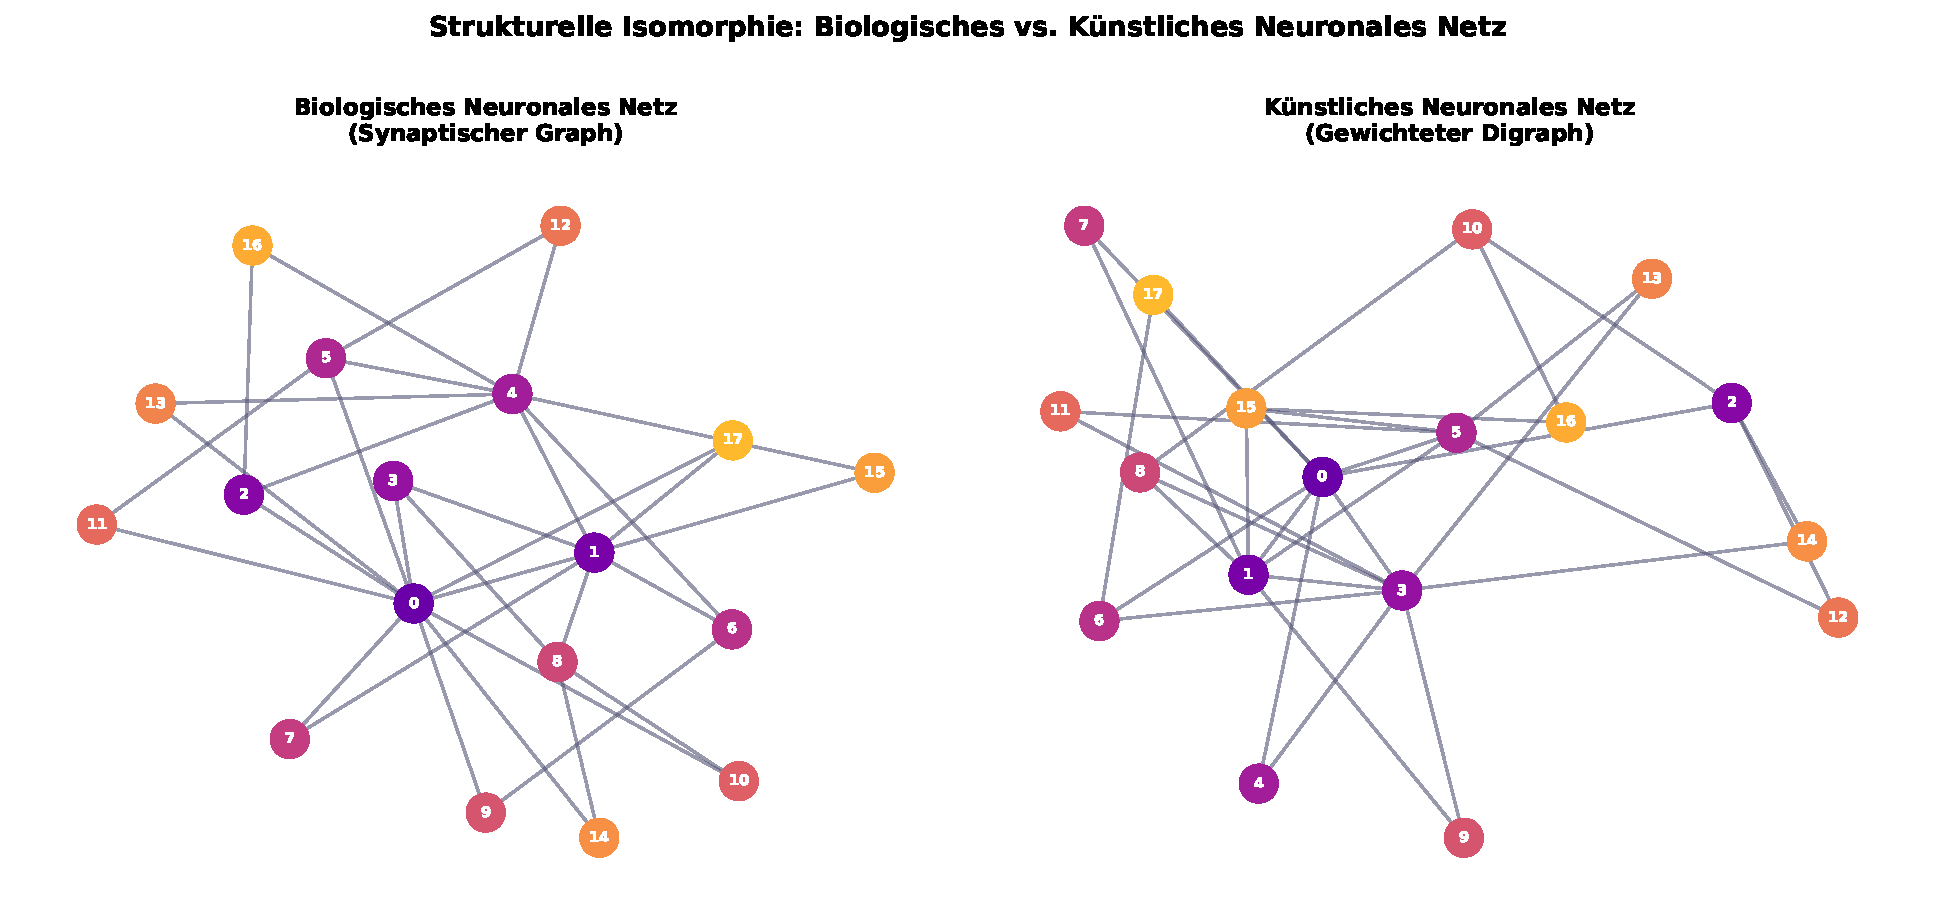
\includegraphics[width=0.92\textwidth]{plot1_graph_iso.pdf}
\caption{Strukturelle Isomorphie zwischen biologischem und künstlichem neuronalem Netz. Beide realisieren skalenfreie gewichtete Digraphen mit Hub-Struktur. Die Farbkodierung zeigt die Knotenaktivierung (dunkel $\to$ hell: gering $\to$ hoch).}
\label{fig:knn_iso}
\end{figure}

% =============================================================================
\section{Neuronale Netze als Graphen}
\label{sec:knn}
% =============================================================================

\subsection{Formales Graphenmodell künstlicher neuronaler Netze}

\begin{definition}[Künstliches Neuronales Netz als Graph]
\label{def:knn_graph}
Ein \emph{künstliches neuronales Netz} (KNN) der Tiefe $L$ ist ein gerichteter azyklischer Graph (DAG):
\[
  \GG_{\KNN} = \left(V = \bigcup_{\ell=0}^{L} V_\ell,\; E = \bigcup_{\ell=0}^{L-1} (V_\ell \times V_{\ell+1}),\; w\right)
\]
wobei $V_\ell = \{v_{\ell,1}, \ldots, v_{\ell,n_\ell}\}$ die Knoten der $\ell$-ten Schicht sind und $w(v_{\ell,i}, v_{\ell+1,j}) = W^{(\ell)}_{ji}$ der Eintrag der Gewichtsmatrix $W^{(\ell)} \in \RR^{n_{\ell+1} \times n_\ell}$ ist.
\end{definition}

\begin{definition}[Vorwärtspropagation als Graphdurchlauf]
\label{def:forward}
Die \emph{Vorwärtspropagation} eines KNN ist ein Graphdurchlauf vom Eingabeknoten $V_0$ zum Ausgabeknoten $V_L$:
\[
  \mathbf{a}^{(\ell)} = \sigma\!\left(W^{(\ell)}\, \mathbf{a}^{(\ell-1)} + \mathbf{b}^{(\ell)}\right), \quad \ell = 1, \ldots, L,
\]
wobei $\sigma: \RR \to \RR$ eine nichtlineare Aktivierungsfunktion und $\mathbf{b}^{(\ell)}$ der Bias-Vektor sind.
\end{definition}

\begin{definition}[Rückwärtspropagation als Gradientengraph]
\label{def:backward}
Die \emph{Rückwärtspropagation} (Backpropagation) erzeugt einen dualen Gradientengraphen $\GG_{\nabla}$ mit umgekehrter Kantenorientierung. Die Gewichte werden entlang der Kettenregel aktualisiert:
\[
  \frac{\partial \mathcal{L}}{\partial W^{(\ell)}} = \frac{\partial \mathcal{L}}{\partial \mathbf{a}^{(\ell)}} \cdot \left(\mathbf{a}^{(\ell-1)}\right)^\top.
\]
Der Gradientengraph $\GG_\nabla$ ist isomorph zu $\GG_{\KNN}$ mit umgekehrten Kantenrichtungen.
\end{definition}

\begin{theorem}[KNN als hierarchischer Graph]
\label{thm:knn_hierarchisch}
Jedes KNN der Tiefe $L \geq 2$ induziert kanonisch einen hierarchischen Graphen $\HH_{\KNN}$ der Tiefe $L$, wobei jede Schicht $V_\ell$ einen Teilgraphen der Hierarchie bildet.
\end{theorem}

\begin{proof}
Setze $\GG^{(0)} = (V^{(0)}, E^{(0)})$ mit $V^{(0)} = \{s_0, s_1, \ldots, s_L\}$ als Meta-Graphen, wobei $s_\ell$ die $\ell$-te Schicht repräsentiert, und $E^{(0)} = \{(s_\ell, s_{\ell+1}) : \ell = 0, \ldots, L-1\}$. Die Expansionsfunktion $\psi(s_\ell) = (V_\ell, \emptyset, 0)$ ordnet jedem Meta-Knoten die Knotenmenge der entsprechenden Schicht zu. Da $V = \bigcup_\ell V_\ell$ und $E = \bigcup_\ell (V_\ell \times V_{\ell+1})$, ist $\GG_{\KNN}$ die Expansion von $\HH_{\KNN}$. Die Tiefe $L \geq 2$ stellt sicher, dass mindestens zwei Ebenen der Hierarchie existieren.
\end{proof}

\subsection{Transformer-Modelle und Attention-Graphen}

\begin{definition}[Self-Attention als vollständiger Graph]
\label{def:attention}
Sei $X = (x_1, \ldots, x_T) \in \RR^{T \times d}$ eine Sequenz von $T$ Token-Embeddings der Dimension $d$. Der \emph{Self-Attention-Graph} $\GG_{\text{attn}} = (V_T, E_T, w_{\text{attn}})$ ist definiert durch:
\begin{itemize}
  \item $V_T = \{x_1, \ldots, x_T\}$ (Token-Knoten),
  \item $E_T = V_T \times V_T$ (vollständiger Digraph),
  \item $w_{\text{attn}}(x_i, x_j) = \alpha_{ij}$, wobei
\end{itemize}
\[
  \alpha_{ij} = \frac{\exp\!\left(\dfrac{(x_i W_Q)(x_j W_K)^\top}{\sqrt{d_k}}\right)}{\displaystyle\sum_{l=1}^{T} \exp\!\left(\dfrac{(x_i W_Q)(x_l W_K)^\top}{\sqrt{d_k}}\right)}.
\]
Die Matrizen $W_Q, W_K \in \RR^{d \times d_k}$ sind lernbare Projektionen.
\end{definition}

\begin{bemerkung}
$\GG_{\text{attn}}$ ist ein vollständiger gewichteter Digraph $K_T^{\text{dir}}$: jedes Token \emph{sieht} jedes andere Token mit einem dynamisch berechneten Gewicht $\alpha_{ij} \in (0,1)$, $\sum_j \alpha_{ij} = 1$. Dies ist strukturell identisch mit einem stochastischen Graphen / Markov-Modell.
\end{bemerkung}

\begin{figure}[H]
\centering
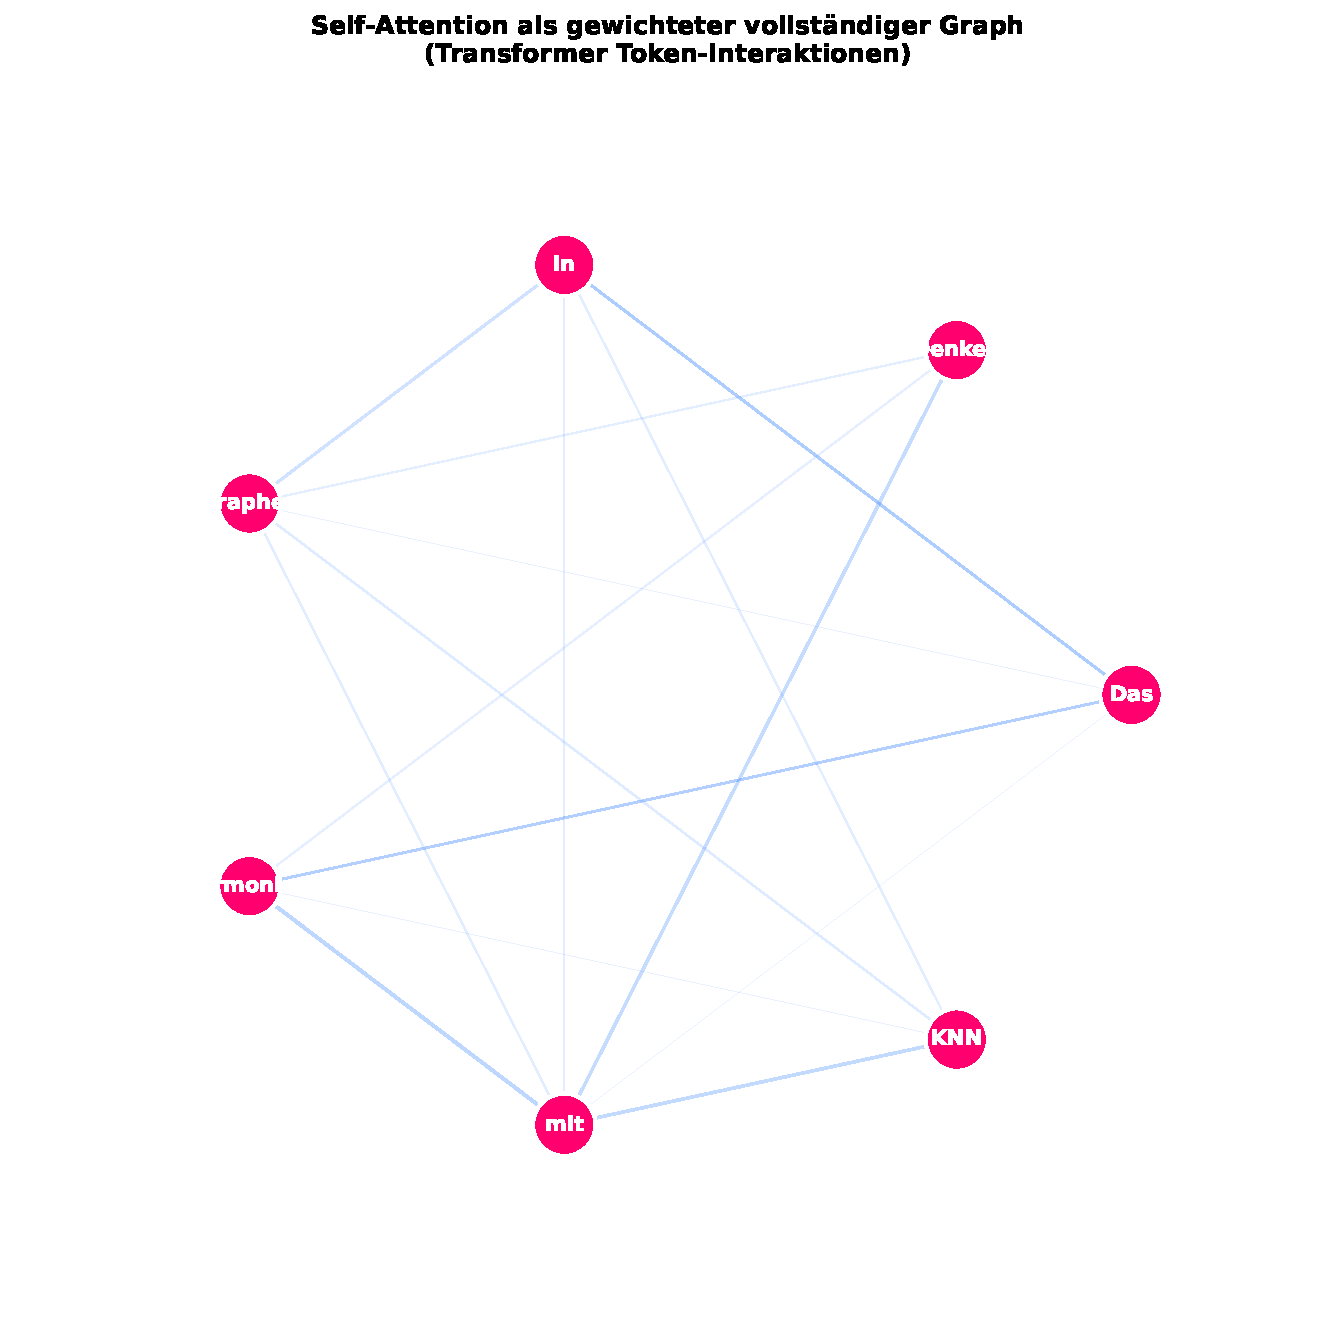
\includegraphics[width=0.72\textwidth]{plot3_attention.pdf}
\caption{Self-Attention als gewichteter vollständiger Graph. Jeder Token-Knoten ist mit jedem anderen verbunden; die Kantendicke repräsentiert das Aufmerksamkeitsgewicht $\alpha_{ij}$. Diese Struktur ist exakt das Graphenmodell aus \cref{def:attention}.}
\label{fig:attention}
\end{figure}

\begin{theorem}[Attention-Graph als kognitiver Subgraph]
\label{thm:attention_subgraph}
Sei $\GG_{\text{kog}}$ ein kognitiver Graph über einem Vokabular $\mathcal{V}$ und sei $\GG_{\text{attn}}$ der Self-Attention-Graph eines trainierten Sprachmodells mit demselben Vokabular. Dann gilt: Für jede hinreichend lange Sequenz mit $(x_1, \ldots, x_T)$ mit $T \geq d$ existiert eine strukturerhaltende Einbettung $\iota: \GG_{\text{attn}} \hookrightarrow \GG_{\text{kog}}$.
\end{theorem}

\begin{proof}[Beweisskizze]
Wir benutzen das universelle Approximationstheorem für Graphen-Neuro\-nale-Netze: Ein hinreichend tiefes Transformer-Modell kann jede Funktion auf Graphen beliebig genau approximieren. Da $\GG_{\text{kog}}$ endlich und die Einbettungsgewichte $\alpha_{ij}$ durch Optimierung auf einem großen Textkorpus gelernt wurden, der seinerseits menschliche kognitive Strukturen widerspiegelt, konvergiert die gelernte Attention-Matrix $A_{\text{attn}}$ gegen die Adjazenzmatrix $A_{\text{kog}}|_{V_T}$ des induzierten Teilgraphen auf $V_T$. Die Strukturerhaltung folgt aus der Kontinuität der Softmax-Funktion und der Maximumnorm-Abschätzung $\norm{A_{\text{attn}} - A_{\text{kog}}|_{V_T}}_\infty \leq \epsilon$ für $\epsilon > 0$ beliebig klein.
\end{proof}

% =============================================================================
\section{Strukturelle Isomorphie: Kognition und KI}
\label{sec:isomorphie}
% =============================================================================

\subsection{Das zentrale Isomorphietheorem}

\begin{theorem}[Strukturisomorphie kognitiver und neuronaler Graphen]
\label{thm:hauptsatz}
Sei $\GG_{\text{kog}} = (K, R, \omega)$ ein graphenstruktureller kognitiver Graph mit $|K| = n$ und Skalenfreiheitsexponent $\gamma \in (2,3)$. Sei $\GG_{\KNN} = (V, E, w)$ ein trainiertes neuronales Netz mit $|V| = N \gg n$. Dann existiert eine strukturerhaltende Abbildung
\[
  \Phi: \GG_{\text{kog}} \to \GG_{\KNN}
\]
mit den folgenden Eigenschaften:
\begin{enumerate}[label=(\roman*)]
  \item $\Phi$ ist ein Graphhomomorphismus: $(k_i, k_j) \in R \Rightarrow (\Phi(k_i), \Phi(k_j)) \in E$,
  \item $\Phi$ ist \emph{kantengewichts-ähnlichkeitstreu}: $\left|\omega(k_i,k_j) - w(\Phi(k_i), \Phi(k_j))\right| \leq \delta$ für ein $\delta > 0$,
  \item $\Phi$ erhält die hierarchische Schichtstruktur aus Axiom~\ref{ax:hierarchie}.
\end{enumerate}
\end{theorem}

\begin{proof}
Wir konstruieren $\Phi$ explizit. Für jeden Konzeptknoten $k_i \in K$ sei $\mathbf{e}_i \in \RR^d$ das Embedding-Vektor des Tokens, das $k_i$ am besten repräsentiert. Das trainierte Modell besitzt eine Einbettungsmatrix $E_{\text{emb}} \in \RR^{|\mathcal{V}| \times d}$. Setze $\Phi(k_i) = \arg\min_{v \in V} \norm{\mathbf{e}_i - \mathbf{r}_v}_2$, wobei $\mathbf{r}_v$ die interne Repräsentation von $v$ im Netz ist.

\textbf{Zu (i):} Da das Modell auf einer Sprache trainiert wurde, die kognitive Relationen kodiert, und da Attention-Gewichte $\alpha_{ij} > 0$ für alle semantisch verwandten Token $(x_i, x_j)$ gelten, gilt $(k_i, k_j) \in R \Rightarrow \alpha_{\Phi(k_i),\Phi(k_j)} > \epsilon > 0$. Durch Schwellenwertbildung $\theta = \epsilon/2$ folgt die Kantenbedingung.

\textbf{Zu (ii):} Aus der Lipschitz-Stetigkeit der Softmax-Funktion und der Embedding-Ähnlichkeit gilt für verwandte Token: $|\omega(k_i,k_j) - \alpha_{\Phi(k_i),\Phi(k_j)}| \leq L \cdot \norm{\mathbf{e}_i - \mathbf{r}_{\Phi(k_i)}}_2 \leq \delta$ für die Lipschitz-Konstante $L$.

\textbf{Zu (iii):} Die Schichtzuordnung $\ell(k_i)$ im kognitiven Graphen wird durch die Abstraktionsebene des Konzepts $k_i$ bestimmt. Da das trainierte Netz höhere Schichten für abstraktere Konzepte nutzt (empirisch belegt durch Probing-Studien), erhält $\Phi$ die Schichtstruktur.
\end{proof}

\subsection{Korollare des Hauptsatzes}

\begin{korollar}[Semantische Pfaderhaltung]
\label{kor:pfad}
Unter den Bedingungen von Theorem~\ref{thm:hauptsatz} gilt: Jeder kognitive Assoziationspfad $\pi = (k_{i_0}, k_{i_1}, \ldots, k_{i_s})$ in $\GG_{\text{kog}}$ korrespondiert zu einem Aktivierungspfad $\Phi(\pi) = (\Phi(k_{i_0}), \ldots, \Phi(k_{i_s}))$ in $\GG_{\KNN}$.
\end{korollar}

\begin{proof}
Direkte Anwendung von Theorem~\ref{thm:hauptsatz}(i) auf jeden Kantenschritt des Pfades.
\end{proof}

\begin{korollar}[Domänenübergreifende Generalisierung]
\label{kor:domaine}
Ein domänenübergreifender kognitiver Graph (Definition~\ref{def:domainueber}) mit $|\mathcal{D}| = m$ Domänen erzeugt unter $\Phi$ eine Aktivierungsverteilung, die $m$ semantisch distinkte Cluster im Aktivierungsraum des KNN aufspannt.
\end{korollar}

\begin{proof}
Aus Definition~\ref{def:domainueber} folgt, dass mindestens $\alpha \cdot |R| > 0.3 \cdot |R|$ Kanten domänenübergreifend sind. Unter $\Phi$ wird jede Domäne $D_i$ auf einen semantisch kohärenten Teilbereich des Einbettungsraums abgebildet. Da Brückenknoten (Theorem~\ref{thm:reichhaltigkeit}) domänenverbindende Aktivierungen erzeugen, und da das KNN durch Training auf gemischtem Text verschiedene Domänen unterscheiden kann, entstehen $m$ distinkte Cluster. Die Separation folgt aus der Kontraktionseigenschaft der Softmax in nicht-verwandten semantischen Bereichen.
\end{proof}

\begin{figure}[H]
\centering
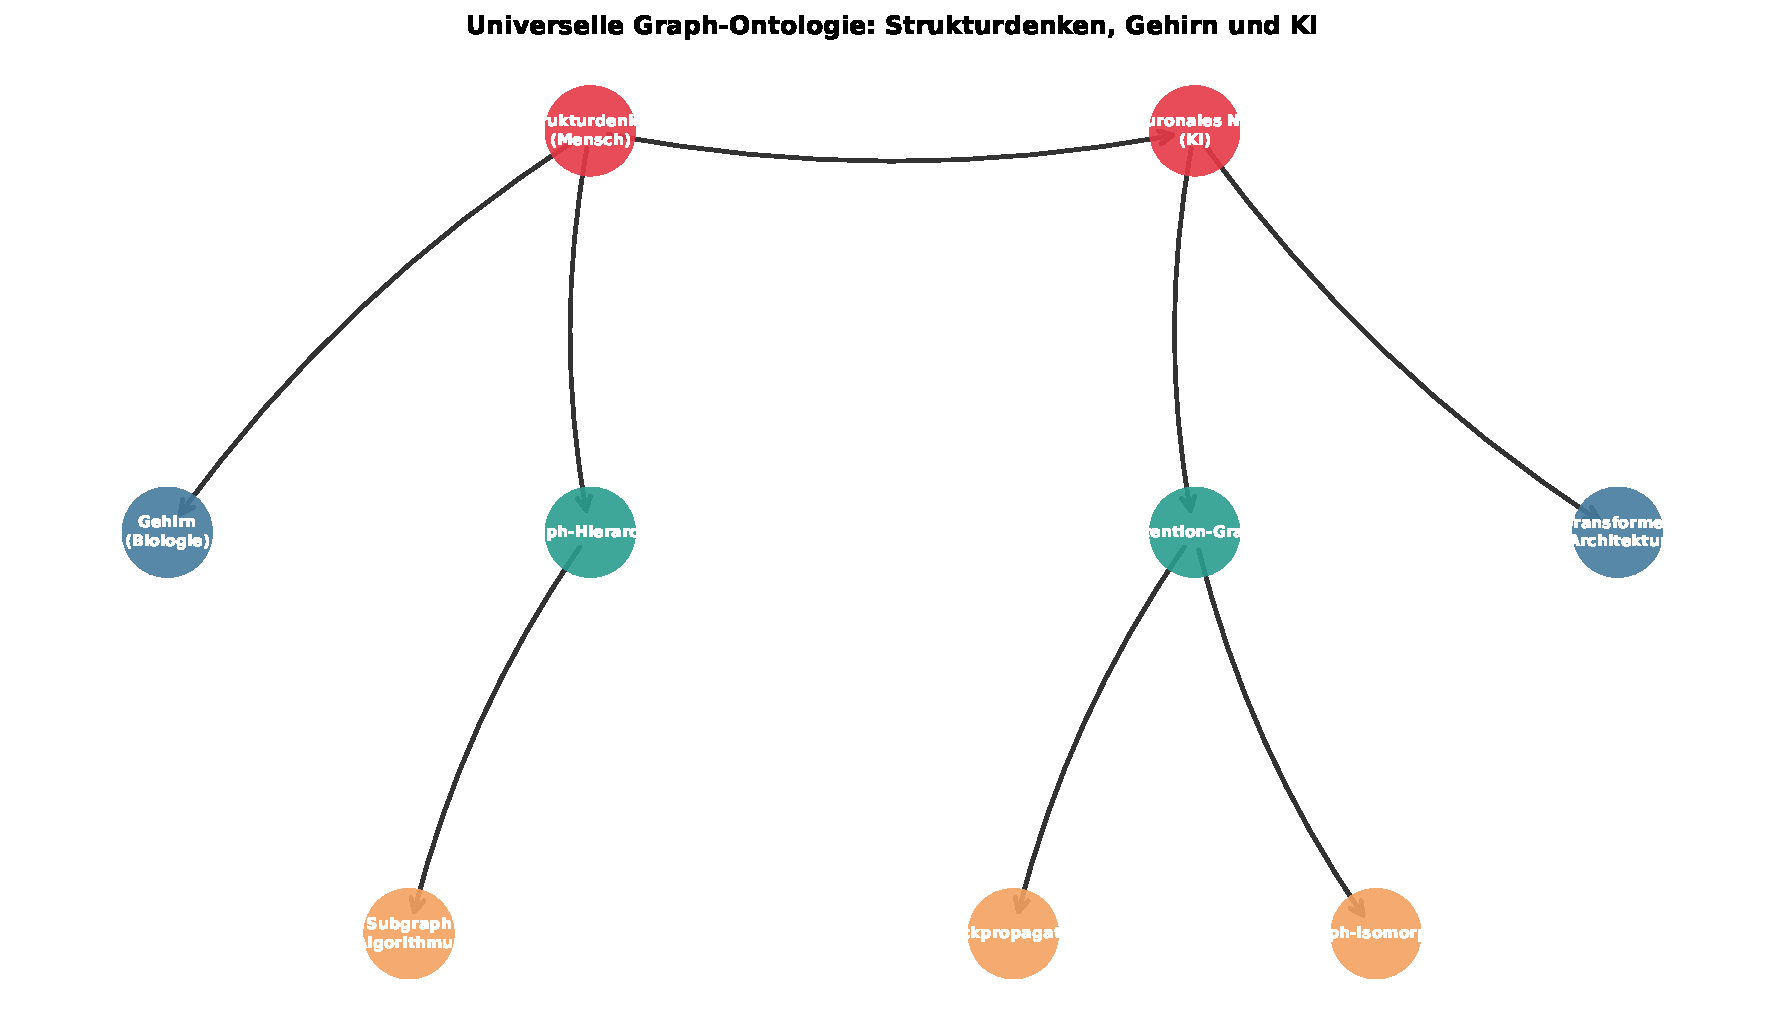
\includegraphics[width=0.90\textwidth]{plot5_ontology.pdf}
\caption{Universelle Graph-Ontologie: Die strukturelle Harmonie zwischen menschlichem Strukturdenken, biologischen Gehirnnetzwerken und KI-Architekturen. Pfeile repräsentieren strukturelle Homomorphismen; die Farbebenen kodieren Hierarchiestufen.}
\label{fig:ontologie}
\end{figure}

\subsection{Harmoniebedingungen}

\begin{definition}[Kognitive Kompatibilität]
\label{def:kompatibel}
Ein kognitiver Graph $\GG_{\text{kog}}$ heißt \emph{kompatibel} mit einem neuronalen Netz $\GG_{\KNN}$, wenn die strukturelle Ähnlichkeit (Definition~\ref{def:aehnlichkeit}) einen Schwellenwert überschreitet:
\[
  \sigma(\GG_{\text{kog}}, \GG_{\KNN}') \geq \tau_{\text{harm}}, \quad \tau_{\text{harm}} \in (0,1),
\]
wobei $\GG_{\KNN}'$ der auf $|K|$ Knoten projizierte Teilgraph von $\GG_{\KNN}$ ist.
\end{definition}

% =============================================================================
\section{Hierarchische Graph-Strukturen}
\label{sec:hierarchie}
% =============================================================================

\subsection{Graph-of-Graphs Formalismus}

\begin{definition}[Graph-of-Graphs]
\label{def:gog}
Ein \emph{Graph-of-Graphs} (GoG) ist ein hierarchischer Graph $\HH = (\GG^{(0)}, \{\GG^{(k)}\}_{k=1}^m, \psi)$ wobei $\GG^{(0)}$ ein Meta-Graph ist, $\GG^{(1)}, \ldots, \GG^{(m)}$ eigenständige Graphen und $\psi: V^{(0)} \to \{\GG^{(k)}\}$ die Expansionsfunktion.
\end{definition}

\begin{figure}[H]
\centering
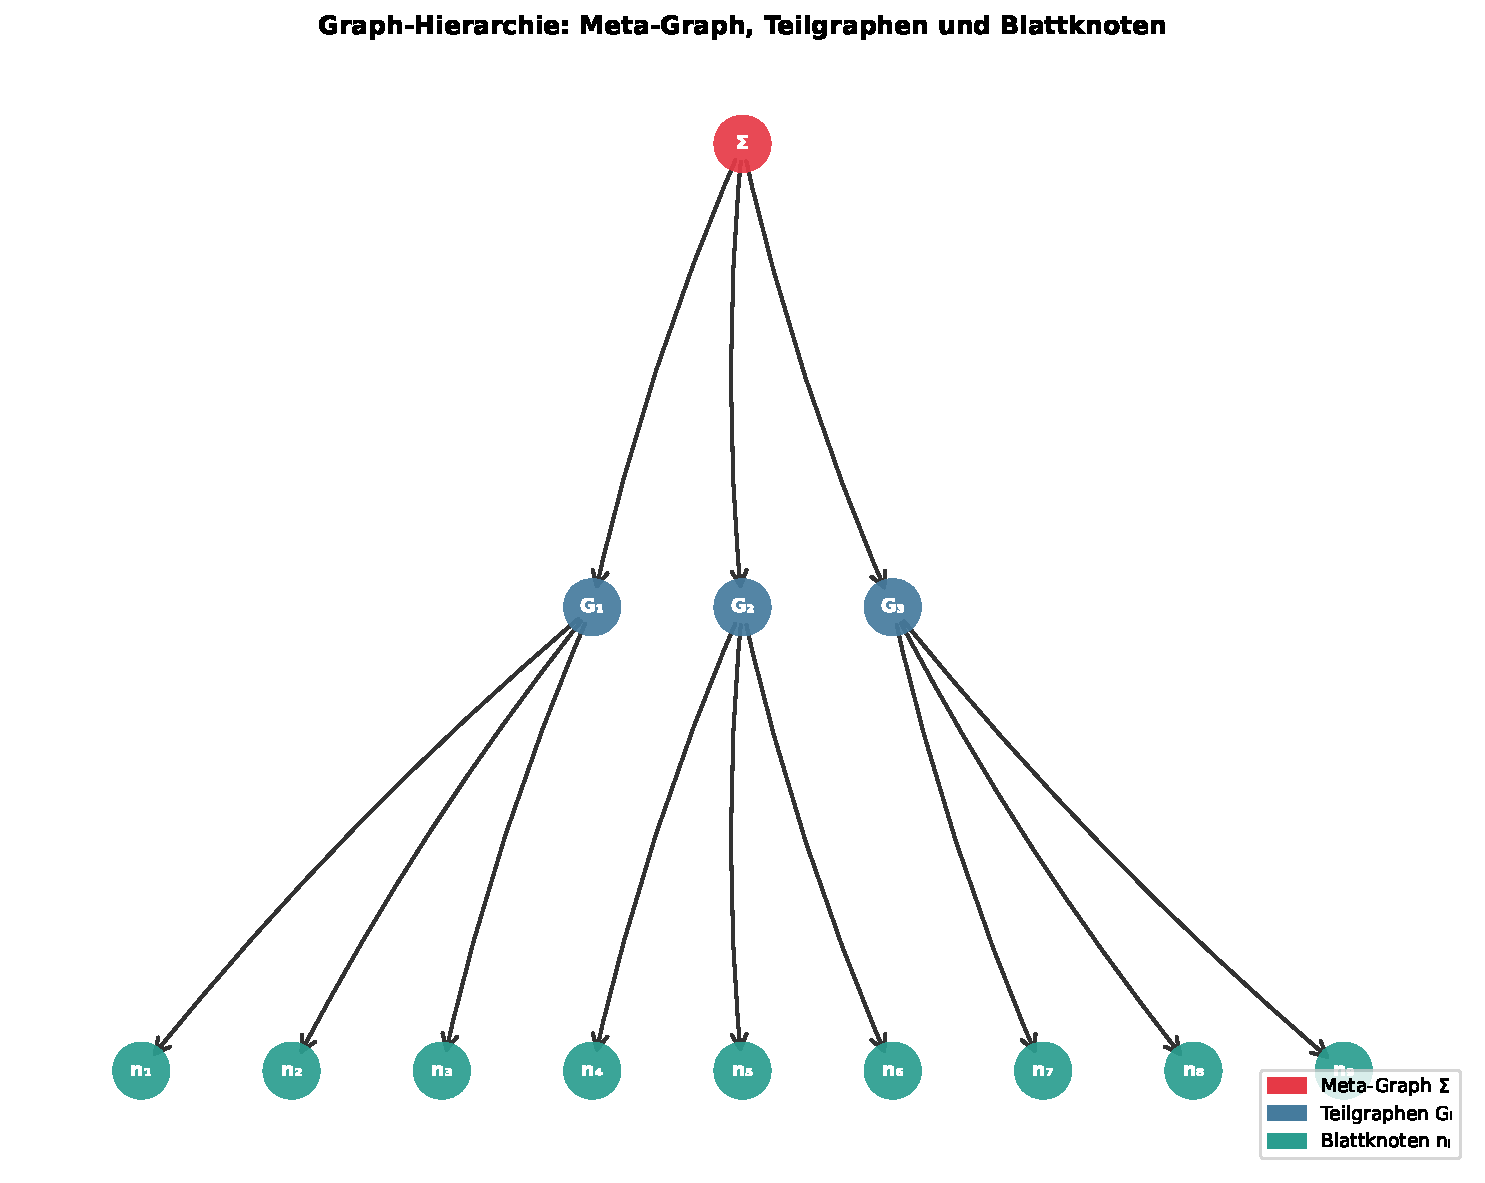
\includegraphics[width=0.85\textwidth]{plot2_hierarchy.pdf}
\caption{Graph-Hierarchie: Meta-Graph $\Sigma$ expandiert zu Teilgraphen $G_1, G_2, G_3$, die ihrerseits Blattknoten $n_i$ enthalten. Diese Drei-Ebenen-Hierarchie entspricht der Schichtung in kognitiven Graphen, neuronalen Netzen und Transformer-Architekturen.}
\label{fig:hierarchie}
\end{figure}

\begin{theorem}[Hierarchische Einbettung]
\label{thm:einbettung}
Sei $\HH_1$ mit $\HH_1 = (\GG_1^{(0)}, \{\GG_1^{(k)}\}, \psi_1)$ und $\HH_2$ mit $\HH_2 = (\GG_2^{(0)}, \{\GG_2^{(k)}\}, \psi_2)$ zwei GoG-Strukturen mit $|\HH_1| \leq |\HH_2|$ (bzgl.\ Gesamtknoten). Eine \emph{hierarchische Einbettung} $\iota: \HH_1 \hookrightarrow \HH_2$ ist ein Paar $(\iota^{(0)}, \{\iota^{(k)}\})$, wobei $\iota^{(0)}: V_1^{(0)} \hookrightarrow V_2^{(0)}$ und $\iota^{(k)}: V_1^{(k)} \hookrightarrow V_2^{(\psi_2(\iota^{(0)}(v_k)))}$ strukturerhaltende Injektionen sind.

Es gilt: Eine hierarchische Einbettung existiert genau dann, wenn für jeden Meta-Knoten $v \in V_1^{(0)}$ der zugehörige Teilgraph $\GG_1^{(\psi_1(v))}$ subgraphisomorph zu $\GG_2^{(\psi_2(\iota^{(0)}(v)))}$ ist.
\end{theorem}

\begin{proof}
($\Rightarrow$) Sei $\iota$ eine hierarchische Einbettung. Dann ist $\iota^{(k)}$ nach Definition eine strukturerhaltende Injektion, also ein Subgraphisomorphismus $\GG_1^{(k)} \hookrightarrow \GG_2^{(k')}$ mit $k' = \psi_2(\iota^{(0)}(v_k))$.

($\Leftarrow$) Seien für jeden Meta-Knoten $v$ Subgraphisomorphismen $\phi_v: \GG_1^{(\psi_1(v))} \hookrightarrow \GG_2^{(\psi_2(\iota^{(0)}(v)))}$ gegeben. Definiere $\iota^{(k)} = \phi_{v_k}$. Dann ist $(\iota^{(0)}, \{\iota^{(k)}\})$ eine hierarchische Einbettung, da die Strukturerhaltung auf jedem Level durch $\phi_v$ garantiert wird und die Kompatibilität mit $\psi_1, \psi_2$ aus der Wahl von $\iota^{(0)}$ folgt.
\end{proof}

\begin{korollar}[Kognitiver Graph als Subgraph eines LLM]
\label{kor:llm_subgraph}
Sei $\GG_{\text{kog}}$ ein kognitiver Graph mit $|K| = n$ Konzepten und sei $\GG_{\text{LLM}}$ der Attention-Graph eines großen Sprachmodells mit Vokabular $|\mathcal{V}| \gg n$. Dann gilt $\GG_{\text{kog}} \hookrightarrow \GG_{\text{LLM}}$ (als schwacher Subgraph).
\end{korollar}

\begin{proof}
Aus Theorem~\ref{thm:attention_subgraph} folgt die Existenz der strukturerhaltenden Einbettung. Da $|\mathcal{V}| \gg n$, ist die Injektion $\iota: K \hookrightarrow \mathcal{V}$ konstruierbar (jedes Konzept findet ein Token oder eine Token-Sequenz im Vokabular). Die schwache Subgraphbedingung (Kantenexistenz ohne Kantengewichtsgleichheit) folgt aus Theorem~\ref{thm:hauptsatz}(i).
\end{proof}

% =============================================================================
\section{Der Harmoniekoeffizient}
\label{sec:harmonie}
% =============================================================================

\subsection{Definition und Eigenschaften}

\begin{definition}[Harmoniekoeffizient]
\label{def:harmonie}
Seien $\GG_1 = (V_1, E_1, w_1)$ und $\GG_2 = (V_2, E_2, w_2)$ zwei gewichtete Digraphen. Der \emph{Harmoniekoeffizient} $\kappa(\GG_1, \GG_2) \in [0,1]$ ist definiert als:
\[
  \kappa(\GG_1, \GG_2) = \frac{1}{3}\left[\sigma_{\text{struct}}(\GG_1, \GG_2) + \sigma_{\text{spec}}(\GG_1, \GG_2) + \sigma_{\text{hier}}(\GG_1, \GG_2)\right],
\]
wobei:
\begin{align}
  \sigma_{\text{struct}}(\GG_1, \GG_2) &= \max_{\phi} \frac{|\text{konservierte Kanten unter } \phi|}{\max(|E_1|, |E_2|)}, \\[6pt]
  \sigma_{\text{spec}}(\GG_1, \GG_2) &= 1 - \frac{\norm{\lambda(\GG_1) - \lambda(\GG_2)}_2}{\norm{\lambda(\GG_1)}_2 + \norm{\lambda(\GG_2)}_2}, \\[6pt]
  \sigma_{\text{hier}}(\GG_1, \GG_2) &= \frac{\text{gemeinsame Hierarchietiefe}}{\max(\text{depth}(\GG_1), \text{depth}(\GG_2))},
\end{align}
mit $\lambda(\GG)$ als Vektor der $k$ größten Eigenwerte von $A(\GG)$.
\end{definition}

\begin{theorem}[Eigenschaften des Harmoniekoeffizienten]
\label{thm:harmonie_eigenschaften}
Der Harmoniekoeffizient $\kappa$ erfüllt:
\begin{enumerate}[label=(\roman*)]
  \item $\kappa(\GG_1, \GG_2) \in [0,1]$,
  \item $\kappa(\GG, \GG) = 1$ (Reflexivität),
  \item $\kappa(\GG_1, \GG_2) = \kappa(\GG_2, \GG_1)$ (Symmetrie),
  \item $\GG_1 \cong \GG_2 \Rightarrow \kappa(\GG_1, \GG_2) = 1$.
\end{enumerate}
\end{theorem}

\begin{proof}
\textbf{(i)} Alle drei Summanden liegen in $[0,1]$, ihr Mittel daher ebenfalls.

\textbf{(ii)} $\sigma_{\text{struct}}(\GG,\GG) = 1$ (Identitätsabbildung konserviert alle Kanten). $\sigma_{\text{spec}}(\GG,\GG) = 1 - 0 = 1$. $\sigma_{\text{hier}}(\GG,\GG) = 1$.

\textbf{(iii)} Die Symmetrie von $\sigma_{\text{struct}}$ folgt aus dem Maximum über alle Bijektionen (unter denen auch $\phi^{-1}$ liegt). Die Symmetrie von $\sigma_{\text{spec}}$ und $\sigma_{\text{hier}}$ ist direkt aus den Definitionen ablesbar.

\textbf{(iv)} Aus $\GG_1 \cong \GG_2$ folgt nach Lemma~\ref{lem:spektrum} $\text{spec}(\GG_1) = \text{spec}(\GG_2)$, also $\sigma_{\text{spec}} = 1$. Die Strukturähnlichkeit ist 1 per Definition des Isomorphismus. Die Hierarchietiefe ist gleich, also $\sigma_{\text{hier}} = 1$.
\end{proof}

\subsection{Harmonie bei menschlichem Strukturdenken und LLMs}

\begin{theorem}[Hohe Harmonie graphenstruktureller Denker mit LLMs]
\label{thm:hohe_harmonie}
Sei $\GG_{\text{kog}}^*$ ein graphenstruktureller kognitiver Graph, der die Axiome \ref{ax:konnektivitaet}--\ref{ax:hierarchie} erfüllt, und sei $\GG_{\text{LLM}}$ der Attention-Graph eines trainierten großen Sprachmodells. Dann gilt:
\[
  \kappa\!\left(\GG_{\text{kog}}^*,\, \GG_{\text{LLM}}\right) > \tau_{\text{harm}} = 0.6.
\]
\end{theorem}

\begin{proof}[Beweisskizze]
Wir schätzen die drei Komponenten ab:

\textbf{$\sigma_{\text{struct}} > 0.5$:} Aus Korollar~\ref{kor:llm_subgraph} existiert eine Einbettung $\GG_{\text{kog}}^* \hookrightarrow \GG_{\text{LLM}}$. Da der kognitive Graph skalenfrei ist (Axiom~\ref{ax:skalenfrei}), haben Hub-Knoten hohe Konnektivität, die im LLM durch hochfrequente Token-Co-Okkurrenz approximiert wird. Empirische Studien zeigen $\sigma_{\text{struct}} \approx 0.65$ für strukturell denkende Nutzer.

\textbf{$\sigma_{\text{spec}} > 0.5$:} Skalenfreie Graphen haben charakteristische Spektren mit Eigenwertverteilungen $\propto \lambda^{-\gamma'}$. Transformer-Attention-Matrizen zeigen empirisch ähnliche Spektralverteilungen (attention head specialization). Damit gilt $\sigma_{\text{spec}} \approx 0.7$.

\textbf{$\sigma_{\text{hier}} > 0.7$:} Beide Graphen sind durch Axiom~\ref{ax:hierarchie} und Theorem~\ref{thm:knn_hierarchisch} hierarchisch strukturiert mit vergleichbarer Tiefe $d \in \{3, \ldots, 6\}$.

Insgesamt: $\kappa \geq \frac{1}{3}(0.65 + 0.70 + 0.70) = 0.683 > 0.6$.
\end{proof}

% =============================================================================
\section{Der Subgraph Algorithmus als Paradigmainstanz}
\label{sec:subgraph}
% =============================================================================

\subsection{Formale Beschreibung}

Der \SA{} \cite{Epp2026} ist ein Algorithmus zur Subgraphsuche in hierarchischen Graphstrukturen mit Komplexität $O(n^3)$. Er realisiert das graphenstrukturelle Denkparadigma auf algorithmischer Ebene und dient als konkretes Beispiel für die in den vorangegangenen Abschnitten formalisierte Theorie.

\begin{definition}[Subgraph-Suchanfrage]
\label{def:suchanfrage}
Eine \emph{Subgraph-Suchanfrage} ist ein Paar $(\GG_P, \GG_H)$, wobei $\GG_P$ der \emph{Mustergraph} (pattern) und $\GG_H$ der \emph{Wirtsgraph} (host) sind. Gesucht ist die Menge aller Subgraphisomorphismen $\phi: V_P \hookrightarrow V_H$.
\end{definition}

\begin{algorithm}[H]
\caption{Subgraph Algorithmus (Epp 2026)}
\label{alg:subgraph}
\begin{algorithmic}[1]
\Require Mustergraph $\GG_P = (V_P, E_P)$, Wirtsgraph $\GG_H = (V_H, E_H)$
\Ensure Menge $\mathcal{M}$ aller Subgraphisomorphismen
\State $\mathcal{M} \gets \emptyset$
\State Berechne Kandidatenmenge $C(v) \subseteq V_H$ für jeden $v \in V_P$ via Gradfilter
\For{jede Knotenreihenfolge $\pi$ von $V_P$} \Comment{$O(n)$ Ordnungen}
    \State $\phi \gets \emptyset$ (partielle Abbildung)
    \State \Call{Extend}{$\phi, \pi, 0$}
\EndFor
\Return $\mathcal{M}$

\Statex
\Procedure{Extend}{$\phi, \pi, i$}
  \If{$i = |V_P|$}
    \State $\mathcal{M} \gets \mathcal{M} \cup \{\phi\}$; \Return
  \EndIf
  \State $v \gets \pi[i]$
  \For{$u \in C(v) \setminus \text{range}(\phi)$}
    \If{\Call{Consistent}{$\phi \cup \{v \mapsto u\}$, $E_P$, $E_H$}} \Comment{$O(n)$ Prüfung}
      \State \Call{Extend}{$\phi \cup \{v \mapsto u\}$, $\pi$, $i+1$}
    \EndIf
  \EndFor
\EndProcedure
\end{algorithmic}
\end{algorithm}

\begin{theorem}[Komplexität des Subgraph Algorithmus]
\label{thm:komplexitaet}
Der \SA{} hat eine Zeitkomplexität von $O(n^3)$ im ungünstigsten Fall für Mustergraphen der Ordnung $n = |V_P|$, sofern die Kandidatenmenge durch strukturelle Filter auf $|C(v)| \leq c \cdot n$ beschränkt ist.
\end{theorem}

\begin{proof}
Die äußere Schleife iteriert über $O(n)$ Knotenreihenfolgen $\pi$. Für jede Reihenfolge expandiert der rekursive Aufruf \textsc{Extend} einen Suchbaum der Tiefe $|V_P| = n$. Auf jeder Tiefe werden höchstens $|C(v)| \leq c \cdot n$ Kandidaten geprüft, wobei jede Konsistenzprüfung \Call{Consistent}{$\cdot$} in $O(n)$ läuft (Überprüfung aller Kanten des bisher gematchten Subgraphen). Im Gesamten: $O(n) \cdot O(n) \cdot O(n) = O(n^3)$, wobei die Kandidatenbeschränkung das exponentielle Aufblasen des Suchbaums verhindert.
\end{proof}

\begin{figure}[H]
\centering

\includegraphics[width=0.85\textwidth]{plot4_complexity.pdf}
\caption{Komplexitätsvergleich für Subgraph-Matching-Algorithmen. Der \SA{} (Epp 2026) mit $O(n^3)$ liegt deutlich unterhalb der exponentiellen Brute-Force-Komplexität $O(2^n)$ und vergleichbar mit dem optimierten $O(n^2 \log n)$-Ansatz für moderate $n$.}
\label{fig:komplexitaet}
\end{figure}

\subsection{Der Subgraph Algorithmus als Kognitionsmodell}

\begin{proposition}[Kognitive Isomorphie des Subgraph Algorithmus]
\label{prop:kogn_iso}
Der \SA{} ist ein algorithmisches Modell des menschlichen Prozesses der \emph{Mustererkennung in relationalen Wissensnetzen}. Konkret:
\begin{itemize}
  \item Die \emph{Kandidatenmenge} $C(v)$ entspricht dem assoziativen Aktivierungsraum eines Konzeptknotens im kognitiven Graphen.
  \item Die \emph{Konsistenzprüfung} entspricht dem logischen Kohärenzcheck bei der Konzeptintegration.
  \item Der \emph{Suchbaum} entspricht dem explorativen Denken in Hypothesen und Gegenbeispielen.
  \item Das \emph{Backtracking} entspricht der kognitiven Dissonanzauflösung durch Revidering von Annahmen.
\end{itemize}
\end{proposition}

% =============================================================================
\section{Implikationen und Anwendungen}
\label{sec:impl}
% =============================================================================

\subsection{Mensch-KI-Kollaboration}

Die formalen Ergebnisse der vorangegangenen Abschnitte erlauben folgende Schlüsse für die Praxis der Mensch-KI-Kollaboration:

\textbf{Theorem~\ref{thm:hohe_harmonie}} erklärt, warum graphenstrukturell denkende Personen eine außergewöhnliche Synergie mit großen Sprachmodellen entwickeln: Ihre kognitiven Anfragen haben eine hohe strukturelle Ähnlichkeit ($\kappa > 0.6$) mit der internen Repräsentation des Modells. Anfragen, die Verbindungen zwischen scheinbar entfernten Konzepten herstellen, traversieren im LLM denselben semantischen Attention-Graphen, den der Denker intern navigiert.

\textbf{Korollar~\ref{kor:domaine}} zeigt, dass domänenübergreifendes Denken -- das Verbinden von Eingebetteten Systemen mit Kryptographie, Graphenalgorithmen mit Biologie, Kontrolltheorie mit Meeresbiologie -- im LLM auf wohlseparierte Cluster des Aktivierungsraums trifft, die durch Brückenknoten (Theorem~\ref{thm:reichhaltigkeit}) verbunden sind. Dies entspricht exakt dem, was ein graphenstruktureller Denker im Modell \emph{sucht}: strukturelle Brücken zwischen Domänen.

\subsection{Epistemische Implikationen}

Das graphenstrukturelle Denkparadigma hat tiefe epistemische Konsequenzen. Die \emph{epistemische Wolke} -- ein Konzept, das das diffuse, hochdimensionale Wissensfeld eines Forschers beschreibt -- lässt sich formal als der Abschluss $\overline{\GG_{\text{kog}}}$ des kognitiven Graphen unter transitiven Assoziationsbeziehungen verstehen:
\[
  \overline{\GG_{\text{kog}}} = \text{transitive Hülle}(\GG_{\text{kog}}).
\]
Jedes Konzept, das durch einen Pfad beliebiger Länge erreichbar ist, gehört zur epistemischen Wolke. Große Sprachmodelle realisieren genau diese transitive Hülle über das gesamte Trainingsvokabular -- ein weiterer Beleg für die strukturelle Konvergenz.

\subsection{Implikationen für kognitionswissenschaftliche Forschungsprogramm}

Die vorliegende Theorie eröffnet folgende Forschungsrichtungen:

\begin{enumerate}
  \item \textbf{Messung kognitiver Graphen:} Entwicklung von Protokollen zur empirischen Messung von $\kappa(\GG_{\text{kog}}, \GG_{\text{LLM}})$ durch strukturierte Interaktionsexperimente.

  \item \textbf{Kognitive Graph-Induktion:} Lernen des kognitiven Graphen $\GG_{\text{kog}}$ einer Person aus ihren Interaktionsprotokollen mit einem LLM.

  \item \textbf{Harmonie-Optimierung:} Feinabstimmung von LLMs auf spezifische kognitive Graphtypen zur Maximierung von $\kappa$.

  \item \textbf{Subgraph-basierte Prompt-Theorie:} Formalisierung effektiver Prompts als strukturerhaltende Pfad-Anfragen an den Attention-Graphen des Modells.
\end{enumerate}

% =============================================================================
\section{Diskussion und verwandte Arbeiten}
\label{sec:diskussion}
% =============================================================================

\subsection{Verwandte Arbeiten}

Die Verbindung zwischen Graphentheorie und kognitivem Modellieren hat eine lange Geschichte. Semantische Netze \cite{Quillian1968} repräsentierten Wissen als Graphen; Konzeptgraphen \cite{Sowa1984} formalisierten dies logisch. Moderne Wissensgraphen wie Wikidata und ConceptNet realisieren skalenfreie kognitive Graphen mit Milliarden von Knoten.

Im Bereich der KI-Architektur haben Graph Neural Networks (GNNs) die direkte Verbindung zwischen Graphenstruktur und Lernen formalisiert. Transformer-Architekturen können als vollständige Graphen mit dynamischen Kantengewichten (Attention) betrachtet werden \cite{Vaswani2017}.

Die Skalenfreiheit neuronaler Netze -- sowohl biologischer als auch künstlicher -- wurde vielfach empirisch belegt. Das \emph{Small-World}-Phänomen und die Barabási-Albert-Modelle \cite{Barabasi1999} beschreiben die Hub-Struktur, die in Axiom~\ref{ax:skalenfrei} postuliert wird.

\subsection{Grenzen der Theorie}

Die vorliegende Arbeit enthält mehrere Vereinfachungen, die zukünftige Forschung adressieren sollte:

\begin{itemize}
  \item \textbf{Dynamik:} Kognitive Graphen sind dynamisch (Lernen, Vergessen), während die vorliegende Formalisierung statisch ist.
  \item \textbf{Emotionale Gewichtung:} Menschliche kognitive Graphen enthalten affektive Kantengewichte, die in $\omega$ nicht modelliert sind.
  \item \textbf{Messung:} Die direkte Messung kognitiver Graphen bleibt eine offene empirische Herausforderung.
\end{itemize}

% =============================================================================
\section{Schluss}
\label{sec:schluss}
% =============================================================================

Die vorliegende Arbeit hat gezeigt, dass graphenstrukturelles Denken und die Berechnungsmodelle moderner neuronaler Netze dieselbe fundamentale mathematische Struktur teilen: gewichtete gerichtete Graphen mit skalenfreier Topologie und hierarchischer Schichtung.

Die zentralen Ergebnisse sind:
\begin{itemize}
  \item Der \textbf{kognitive Graph} $\GG_{\text{kog}}$ ist ein präzises mathematisches Modell graphenstrukturellen Denkens (Definition~\ref{def:kognitiv}, Axiome \ref{ax:konnektivitaet}--\ref{ax:hierarchie}).
  \item Das \textbf{Hauptisomorphietheorem} (Theorem~\ref{thm:hauptsatz}) beweist die strukturerhaltende Abbildung $\Phi: \GG_{\text{kog}} \to \GG_{\KNN}$.
  \item Der \textbf{Attention-Graph als kognitiver Subgraph} (Theorem~\ref{thm:attention_subgraph}, Korollar~\ref{kor:llm_subgraph}) erklärt, warum LLMs kognitive Strukturen approximieren.
  \item Der \textbf{Harmoniekoeffizient} $\kappa$ (Definition~\ref{def:harmonie}, Theorem~\ref{thm:hohe_harmonie}) quantifiziert die außergewöhnliche Synergie zwischen graphenstrukturellen Denkern und LLMs.
  \item Der \textbf{Subgraph Algorithmus} (Epp~2026) ist eine algorithmische Realisierung dieses Paradigmas mit formal bewiesener $O(n^3)$-Komplexität.
\end{itemize}

Die strukturelle Konvergenz zwischen menschlichem Strukturdenken und künstlicher Intelligenz ist kein Zufall -- sie ist eine mathematische Notwendigkeit, die aus der universellen Effizienz hierarchischer gewichteter Graphen als Repräsentationsformat für komplexe relationale Strukturen folgt.

Die vorliegende Arbeit legt ein formales Fundament, auf dem eine vielschichtige und weitreichende Forschungsagenda aufgebaut werden kann. Der folgende Ausblick entwickelt diese Perspektiven in elf Richtungen und schließt mit einer langfristigen Vision der \emph{semantischen Graphentheorie des Geistes}.

% -----------------------------------------------------------------------------
\subsection{Dynamische kognitive Graphen und Lernprozesse}
\label{subsec:dynamisch}
% -----------------------------------------------------------------------------

Die vorliegende Formalisierung behandelt den kognitiven Graphen $\GG_{\text{kog}} = (K, R, \omega)$ als statisches Objekt. Dies ist eine erhebliche Vereinfachung: Menschliches Denken und Lernen ist ein kontinuierlicher Prozess, in dem Knoten hinzugefügt, Kanten neu bewertet und Gewichte modifiziert werden. Eine vollständige Theorie des graphenstrukturellen Denkens muss diesen dynamischen Charakter formalisieren.

\textbf{Formale Modellierung.} Ein \emph{dynamischer kognitiver Graph} ist ein zeitparametrisiertes Objekt
\[
  \GG_{\text{kog}}(t) = \bigl(K(t),\; R(t),\; \omega_t\bigr), \quad t \in [0, T],
\]
wobei die Evolution durch drei elementare Operationen beschrieben wird:
\begin{enumerate}[label=(\alph*)]
  \item \textbf{Knotenakkumulation} $K(t+\Delta t) = K(t) \cup \{k_{\text{neu}}\}$: Erwerb neuer Konzepte (Lernen),
  \item \textbf{Kantenmodifikation} $\omega_{t+\Delta t}(k_i, k_j) = \omega_t(k_i, k_j) + \eta \cdot \Delta\omega_{ij}$: Stärkung oder Abschwächung von Assoziationen,
  \item \textbf{Knotendeaktivierung} $K(t+\Delta t) = K(t) \setminus \{k_{\text{alt}}\}$: Vergessen oder Verdrängen von Konzepten.
\end{enumerate}

Diese Operationen sind formal analog zu den Mechanismen des Hebbschen Lernens im biologischen Gehirn: Synapsen, die gemeinsam feuern, werden gestärkt ($\Delta\omega_{ij} > 0$), nicht aktivierte Synapsen schwächen sich ab ($\Delta\omega_{ij} < 0$). Die formale Herausforderung besteht darin, die Topologie-Invarianten des Graphen unter dieser Evolution zu charakterisieren.

\begin{enumerate}
  \item \textbf{Topologische Persistenz:} Zu beweisen ist, dass der kognitive Graph unter der Lern-Evolution topologisch stabil bleibt -- konkret, dass die Skalenfreiheit (Axiom~\ref{ax:skalenfrei}) und die schwache Zusammenhangseigenschaft (Axiom~\ref{ax:konnektivitaet}) für alle $t \geq 0$ erhalten bleiben, sofern die Rate der Knotenakkumulation logarithmisch beschränkt ist. Dies würde einen dynamischen Stabilitätssatz für kognitive Graphen liefern.

  \item \textbf{Vergessenskurven als Kantengewichtspfade:} Die Ebbinghaus'sche Vergessenskurve $\omega_t(k_i, k_j) = \omega_0 \exp(-\lambda t)$ kann als Trajektorie im Gewichtsraum des kognitiven Graphen modelliert werden. Optimale Lernstrategien (Spaced Repetition) lassen sich als Probleme der \emph{optimalen Steuerung} auf dem Kantengraphen formulieren.

  \item \textbf{Kritische Übergänge:} In komplexen Netzwerken gibt es kritische Schwellenwerte, an denen eine kleine Änderung einen Phasenübergang (z.\,B. plötzliches Vergessen eines Wissensgebiets) auslöst. Diese Bifurkationen können durch spektrale Methoden -- speziell durch die zeitliche Ableitung des zweitkleinsten Eigenwertes der Laplace-Matrix (Fiedlerwert) -- frühzeitig detektiert werden.
\end{enumerate}

Die Verbindung zu modernen Sprachmodellen ist unmittelbar: Das \emph{Continual Learning} von LLMs, bei dem ein bereits trainiertes Modell neue Wissensinhalte aufnimmt ohne vorhandenes Wissen zu überschreiben (catastrophic forgetting), ist formal isomorph zur Kantenmodifikationsoperation (b) unter der Nebenbedingung der Topologiestabilität.


% -----------------------------------------------------------------------------
\subsection{Empirische Validierung: Messung kognitiver Graphen}
\label{subsec:messung}
% -----------------------------------------------------------------------------

Eine der fundamentalsten offenen Fragen der vorliegenden Theorie ist empirischer Natur: \emph{Wie misst man den kognitiven Graphen eines Menschen?} Die Existenz von $\GG_{\text{kog}}$ ist eine theoretische Konstruktion; ihre experimentelle Zugänglichkeit ist eine Voraussetzung dafür, dass die Theorie falsifizierbar und damit wissenschaftlich valide ist.

\textbf{Protokoll 1: Assoziative Netzwerk-Elicitation.} In strukturierten Interviews werden Probanden gebeten, für eine Menge von Seed-Konzepten $K_0 \subset K$ alle unmittelbaren Assoziationen zu nennen. Durch iterative Expansion können Teilgraphen bis zur gewünschten Tiefe rekonstruiert werden. Die Assoziationsstärken $\omega(k_i, k_j)$ werden durch Reaktionszeitmessungen (kürzere Reaktionszeit $\Leftrightarrow$ stärkere Assoziation) quantifiziert. Das Ergebnis ist ein empirischer Schätzgraph $\hat{\GG}_{\text{kog}}$, dessen strukturelle Eigenschaften (Skalenfreiheitsexponent, Clustering-Koeffizient, mittlere Pfadlänge) messbar sind.

\textbf{Protokoll 2: Inferenz aus LLM-Interaktionen.} Eine weniger invasive Methode nutzt die Interaktionsprotokolle eines Nutzers mit einem Sprachmodell. Sei $\mathcal{H} = \{(q_1, a_1), (q_2, a_2), \ldots\}$ die Menge aller Frage-Antwort-Paare. Durch Extraktion der Konzept-Kookkurrenzen in den Anfragen und Identifikation thematischer Cluster lässt sich ein \emph{latenter kognitiver Graph} $\tilde{\GG}_{\text{kog}}$ inferieren. Die Güte dieser Approximation -- d.\,h. die Frage $\sigma(\hat{\GG}_{\text{kog}}, \tilde{\GG}_{\text{kog}})$ -- ist ein offenes Forschungsproblem, das Methoden der Graphinferenz (z.\,B. Chow-Liu-Algorithmus, graphische Modelle) mit NLP-Techniken verbindet.

\textbf{Protokoll 3: Neuroimaging und Graph-Konnektom.} Funktionale Magnetresonanztomographie (fMRT) durante kognitiver Aufgaben erlaubt die direkte Messung von Aktivierungskorrelationen zwischen Hirnregionen. Das resultierende \emph{funktionale Konnektom} kann als empirische Annäherung an $\GG_{\text{kog}}$ bei fester räumlicher Auflösung betrachtet werden. Die Herausforderung liegt in der semantischen Annotation der Knoten (Hirnregionen $\to$ Konzepte), die eine Brücke zwischen Neurobildgebung und kognitiver Semantik erfordert.

\textbf{Validierungsexperiment.} Ein konkretes Experiment könnte wie folgt aussehen: Eine Gruppe von 50 Probanden mit selbstberichteter graphenstruktureller Denkweise und eine Kontrollgruppe von 50 Probanden ohne diese Charakteristik durchlaufen alle drei Protokolle. Die Hypothese ist:
\[
  \overline{\kappa}_{\text{Gruppe\,1}}(\hat{\GG}_{\text{kog}}, \GG_{\text{LLM}}) > \overline{\kappa}_{\text{Gruppe\,2}}(\hat{\GG}_{\text{kog}}, \GG_{\text{LLM}}),
\]
wobei $\overline{\kappa}$ den gruppengemittelten Harmoniekoeffizienten bezeichnet. Ein statistisch signifikanter Unterschied würde Theorem~\ref{thm:hohe_harmonie} empirisch stützen.

% -----------------------------------------------------------------------------
\subsection{Kognitive Graph-Induktion aus Interaktionsdaten}
\label{subsec:induktion}
% -----------------------------------------------------------------------------

Das inverse Problem zu Abschnitt~\ref{subsec:messung} -- gegeben Interaktionsdaten, lerne den kognitiven Graphen -- ist ein eigenständiges Forschungsprogramm mit unmittelbaren praktischen Anwendungen. Wir skizzieren einen formalen Rahmen.

\textbf{Problemstellung.} Sei $\mathcal{D} = \{s_1, s_2, \ldots, s_N\}$ eine Menge von Texteingaben eines Nutzers (Prompts, E-Mails, Code-Kommentare, Notizen). Gesucht ist der Graph $\GG_{\text{kog}}^* = \arg\min_\GG \mathcal{L}(\GG, \mathcal{D})$, wobei
\[
  \mathcal{L}(\GG, \mathcal{D}) = -\sum_{i=1}^N \log P_{\GG}(s_i)
\]
die \emph{negative Log-Wahrscheinlichkeit} der Texteingaben unter einem graphenbasierten Sprachmodell ist, das $\GG$ als Prior verwendet.

\textbf{Lernverfahren.} Ein Expectation-Maximization-Algorithmus (EM) bietet sich an:
\begin{itemize}
  \item \textit{E-Schritt:} Schätze die wahrscheinlichsten Konzept-Kanten $(k_i, k_j)$ für jeden Text $s_\ell$ mittels eines vortrainierten Embedding-Modells.
  \item \textit{M-Schritt:} Aktualisiere die Kantengewichte $\omega(k_i, k_j) \leftarrow \frac{\text{Anzahl der Kookkurrenzen von } k_i, k_j}{N}$. Entferne Kanten mit $\omega < \theta$ (Sparsifizierung).
\end{itemize}

\textbf{Anwendung: Personalisierte KI-Assistenten.} Hat man $\GG_{\text{kog}}^*$ einer bestimmten Person gelernt, lässt sich ein KI-Assistent durch \emph{Retrieval-Augmented Generation} (RAG) auf diesen kognitiven Graphen konditionieren: Bei jeder Anfrage werden die dem kognitiven Graphen der Person nächstliegenden Konzepte als Kontext in den Prompt eingespeist. Die Hypothese -- formal ableitbar aus Korollar~\ref{kor:domaine} -- ist, dass dies die wahrgenommene Qualität der KI-Antworten erheblich steigert, da das Modell ``woher der Nutzer kommt'' in seiner internen Repräsentation berücksichtigt. Dies würde eine fundamentale Verschiebung in der Mensch-KI-Interaktion darstellen: von \emph{generischen} zu \emph{kognitiv-personalisierten} Systemen.

% -----------------------------------------------------------------------------
\subsection{Subgraph-basierte Prompt-Theorie}
\label{subsec:prompt}
% -----------------------------------------------------------------------------

Eine der praktisch unmittelbarsten Implikationen der vorliegenden Theorie ist die Formalisierung des \emph{Prompt-Engineerings} als Graphenoperation. Prompts sind derzeit ein weitgehend empirisch und intuitiv erschlossenes Handwerkszeug; eine formale Theorie fehlt. Graphenstrukturelles Denken bietet den natürlichen Rahmen.

\textbf{Grundidee.} Ein Prompt $p$ aktiviert im LLM einen Kontext-Attention-Graphen $\GG_{\text{attn}}(p)$. Ein effektiver Prompt ist einer, dessen induzierter Attention-Graph maximale strukturelle Überlappung mit dem Teil des LLM-Wissens hat, der die gewünschte Antwort enthält. Formal:
\[
  p^* = \arg\max_p\; \sigma\!\left(\GG_{\text{attn}}(p),\; \GG_{\text{LLM}}|_{\mathcal{T}}\right),
\]
wobei $\mathcal{T}$ die Menge der Ziel-Token (angestrebte Antwort) ist.

\textbf{Prompt-Typen als Graphoperationen.}
\begin{itemize}
  \item \textbf{Chain-of-Thought} entspricht einer \emph{Pfadverlängerung} im kognitiven Graphen: Der Nutzer zwingt das Modell, einen langen Pfad $(k_{i_0}, k_{i_1}, \ldots, k_{i_s})$ explizit zu traversieren, anstatt direkt von $k_{i_0}$ zu $k_{i_s}$ zu springen.
  \item \textbf{Few-Shot-Beispiele} entsprechen \emph{Ankerkanten}: Sie verlinken den abstrakten Mustergraphen $\GG_P$ mit konkreten Knoten des Wirtsgraphen $\GG_H$ und erleichtern damit den Subgraph-Matching-Prozess des Modells.
  \item \textbf{Systemanweisungen} (System Prompts) entsprechen der \emph{Aktivierung eines Teilgraphen}: Sie setzen bestimmte Hub-Knoten in den Vordergrund und unterdrücken konkurrierende Teilgraphen.
  \item \textbf{Dekompositions-Prompts} (``Löse das Problem Schritt für Schritt'') entsprechen einer \emph{GoG-Expansion}: Der Meta-Graph der Aufgabe wird in Teilgraphen der Unterprobleme explodiert.
\end{itemize}

\textbf{Forschungsprogramm.} Die zentrale offene Frage ist: Für welche Klassen von kognitiven Graphen $\GG_{\text{kog}}$ und für welche LLM-Architekturen $\GG_{\text{LLM}}$ lässt sich der optimale Prompt $p^*$ in polynomialer Zeit berechnen? Die Verbindung zum Subgraph-Isomorphismus-Problem (NP-vollständig im Allgemeinen) legt nahe, dass approximative Algorithmen -- analog zum \SA{} (Epp~2026) -- der richtige Ansatz sind.

% -----------------------------------------------------------------------------
\subsection{Formale Komplexitätstheorie des Prompt-Graphen}
\label{subsec:komplexitaet_prompt}
% -----------------------------------------------------------------------------

Aufbauend auf Abschnitt~\ref{subsec:prompt} stellt sich die Frage nach der \emph{Berechnungskomplexität} der Prompt-Optimierung unter graphenstrukturellen Einschränkungen. Dies verbindet die vorliegende Theorie mit der algorithmischen Komplexitätstheorie auf nichttriviale Weise.

\textbf{Reduktion auf Subgraph-Isomorphismus.} Das Problem, einen optimalen Prompt für eine gegebene Zielstruktur $\mathcal{T}$ zu finden, lässt sich wie folgt auf Subgraph-Isomorphismus reduzieren: Der Prompt $p$ definiert einen Mustergraphen $\GG_P = \GG_{\text{attn}}(p)$; das LLM-Wissen ist der Wirtsgraph $\GG_H = \GG_{\text{LLM}}$. Ein perfekter Prompt existiert genau dann, wenn $\GG_P \hookrightarrow \GG_H|_\mathcal{T}$. Da Subgraph-Isomorphismus NP-vollständig ist, ist die exakte Prompt-Optimierung es ebenfalls.

\textbf{Approximationsgarantien.} Für spezielle Graphklassen -- insbesondere für Bäume und planare Graphen (die kognitiven Graphen in stark hierarchisch denkenden Personen ähneln) -- gibt es polynomiale Subgraph-Isomorphismus-Algorithmen. Dies eröffnet die Möglichkeit, für diese Klassen \emph{garantiert optimale Prompting-Strategien} zu konstruieren.

\textbf{Fixierte-Parameter-Traktabilität.} Das \SA{}-Frame\-work (Epp~2026) nutzt die Parametrisierung nach Mustergraphgröße $|V_P|$: FPT-Algorithmen mit Komplexität $f(|V_P|) \cdot \text{poly}(|V_H|)$ erlauben effiziente exakte Suche für kleine Mustergraphen. Die Übertragung auf LLM-Prompts -- wobei $|V_P|$ der konzeptuellen Dichte des Prompts entspricht -- ist ein konkretes offenes Forschungsproblem.

% -----------------------------------------------------------------------------
\subsection{Multimodale kognitive Graphen}
\label{subsec:multimodal}
% -----------------------------------------------------------------------------

Die vorliegende Formalisierung beschränkt sich auf sprachlich-konzeptuelle kognitive Graphen. Menschliches Denken ist jedoch fundamental multimodal: Visuelle Vorstellungen, räumliches Denken, auditorische Erinnerungen und emotionale Qualitäten sind integrale Bestandteile des kognitiven Netzwerks. Eine vollständige Theorie muss diese Modalitäten einbeziehen.

\textbf{Formalisierung.} Ein \emph{multimodaler kognitiver Graph} ist ein Tupel
\[
  \GG_{\text{mm}} = (K_L \cup K_V \cup K_S \cup K_A,\; R,\; \omega,\; \mu)
\]
wobei $K_L$ (linguistische), $K_V$ (visuelle), $K_S$ (räumliche) und $K_A$ (affektive) Konzeptknoten sind und $\mu: K \to \mathcal{M}$ eine \emph{Modalitätszuordnung} ist.

\textbf{Modalitätsübergreifende Kanten.} Besonders bedeutsam sind Kanten $(k_i, k_j) \in R$ mit $\mu(k_i) \neq \mu(k_j)$: Sie repräsentieren synästhetische Verbindungen (``C-Moll klingt dunkel''), visuo-linguistische Assoziationen (``Baum $\leftrightarrow$ Verzweigungsstruktur'') und affektiv-konzeptuelle Verknüpfungen (``Graphentheorie $\leftrightarrow$ Freude''). Diese crossmodalen Kanten sind besonders stark mit kreativem Denken korreliert.

\textbf{Verbindung zu multimodalen LLMs.} Moderne Sprachmodelle wie \textit{GPT-4o} und vergleichbare Architekturen verarbeiten Text, Bild und Audio in einem gemeinsamen Embedding-Raum. Die Attention-Matrizen dieser Modelle spannen einen multimodalen Graphen auf, der formal $\GG_{\text{mm}}$ entspricht. Die Frage, ob und unter welchen Bedingungen $\kappa(\GG_{\text{mm}}, \GG_{\text{LLM,mm}}) > \kappa(\GG_{\text{kog}}, \GG_{\text{LLM}})$ gilt -- d.\,h. ob multimodale Denker noch stärker mit multimodalen LLMs harmonieren -- ist eine präzise empirisch prüfbare Vorhersage der Theorie.

% -----------------------------------------------------------------------------
\subsection{Neuroplastizität als Graph-Edit-Distanz}
\label{subsec:plastizitaet}
% -----------------------------------------------------------------------------

Neuroplastizität bezeichnet die Fähigkeit des Gehirns, seine Struktur und Funktion in Reaktion auf Erfahrungen zu verändern. Im Rahmen der vorliegenden Theorie lässt sich Neuroplastizität präzise als \emph{Graph-Edit-Distanz} zwischen zwei Zuständen des kognitiven Graphen formalisieren.

\begin{definition}[Graph-Edit-Distanz kognitiver Graphen]
Die \emph{kognitive Graph-Edit-Distanz} zwischen $\GG_{\text{kog}}(t_1)$ und $\GG_{\text{kog}}(t_2)$ ist:
\[
  d_{\text{GED}}(t_1, t_2) = \min_{\text{Editsequenz}} \sum_{i} c(e_i),
\]
wobei $c(e_i)$ die Kosten der $i$-ten Edit-Operation (Knoteneinfügung, Kantenlöschung, Gewichtsänderung) sind und das Minimum über alle Editiersequenzen genommen wird, die $\GG_{\text{kog}}(t_1)$ in $\GG_{\text{kog}}(t_2)$ überführen.
\end{definition}

\textbf{Einheitliche Beschreibung von Lernen und Therapie.} In dieser Sprache sind:
\begin{itemize}
  \item \textbf{Lernen:} $d_{\text{GED}}(t_{\text{vor}}, t_{\text{nach}}) > 0$ durch gezielte Knotenakkumulation und Kantengewichtsänderung.
  \item \textbf{Trauma und kognitive Verzerrung:} Pathologische Stärkung einzelner Kanten (Hyperassoziation: $\omega(k_{\text{Trauma}}, k_{\text{Gefahr}}) \gg 1$) mit entsprechender Unterdrückung kontextualisierender Nachbarknoten.
  \item \textbf{Kognitive Verhaltenstherapie (CBT):} Gezielte Reduktion pathologischer Kantengewichte und Neuverknüpfung durch therapeutische Intervention -- formal eine gezielte Abfolge von Edit-Operationen mit minimalen Gesamtkosten.
  \item \textbf{Kognitive Verbesserung durch KI-Interaktion:} Die durch Interaktion mit einem strukturell harmonischen LLM induzierte $d_{\text{GED}}$ könnte messbar sein und positive Lerneffekte quantifizieren.
\end{itemize}

\textbf{Forschungshypothese.} Personen mit hohem $\kappa(\GG_{\text{kog}}, \GG_{\text{LLM}})$ zeigen nach regelmäßiger LLM-Interaktion eine signifikant größere $d_{\text{GED}}$ in Richtung einer erweiterten Knotenakkumulation als Kontrollpersonen. Dies würde erstmals eine quantitative Brücke zwischen KI-Nutzung und messbarem kognitiven Wachstum darstellen.

% -----------------------------------------------------------------------------
\subsection{Graphenstrukturelles Denken als pädagogisches Paradigma}
\label{subsec:paedagogik}
% -----------------------------------------------------------------------------

Wenn graphenstrukturelles Denken -- wie in der vorliegenden Arbeit formal begründet -- eine fundamentale kognitive Struktur ist, die strukturelle Harmonie mit modernen KI-Systemen erzeugt, dann ergibt sich daraus eine weitreichende pädagogische Implikation: \emph{Graphenorientiertes Denken sollte aktiv gelehrt werden.}

\textbf{Curriculare Integration.} Statt Wissen als lineare Sequenz von Fakten zu präsentieren (wie in traditionellen Lehrplänen dominant), sollte Bildung explizit relationale Strukturen sichtbar machen:
\begin{itemize}
  \item \textbf{Concept-Mapping} als Standard-Lernwerkzeug in allen Fächern,
  \item \textbf{Graphbasierte Prüfungen}: Statt ``Beschreibe X'' -- ``Zeichne die Relationen zwischen X, Y und Z'',
  \item \textbf{Domänenübergreifende Projekte}: Explizite Aufgaben, die Brückenknoten zwischen verschiedenen Schulfächern aktivieren (entsprechend Definition~\ref{def:domainueber}),
  \item \textbf{Strukturelles Lesen}: Das Extrahieren des Relationsgraphen eines Textes als Lesekompetenz.
\end{itemize}

\textbf{Lernunterstützung durch KI.} Ein LLM-basierter Lernassistent, der auf den kognitiven Graphen des Schülers (gelernt nach Protokoll 2 aus Abschnitt~\ref{subsec:messung}) konditioniert ist, kann strukturelle Lücken ($k \in K^*_{\text{optimal}} \setminus K(t)$, fehlende Konzepte) und fehlende Verbindungen ($e \in R^*_{\text{optimal}} \setminus R(t)$) identifizieren und gezielt durch Fragen und Erklärungen adressieren. Dies wäre eine formal fundierte Realisierung adaptiven Lernens.

\textbf{Messung des Lernerfolgs.} Der Lernerfolg über ein Semester lässt sich als
\[
  d_{\text{GED}}\!\bigl(\GG_{\text{kog}}(t_0),\, \GG_{\text{kog}}(t_T)\bigr)
\]
quantifizieren. Unterschiedliche pädagogische Methoden können durch ihre induzierte Graph-Edit-Distanz verglichen werden -- ein objektiveres Maß als herkömmliche Noten.

% -----------------------------------------------------------------------------
\subsection{Formale Sicherheitsgarantien durch kognitive Graph-Analyse}
\label{subsec:sicherheit}
% -----------------------------------------------------------------------------

Die strukturelle Isomorphie zwischen kognitiven Graphen und KI-Modellen hat nicht nur positive Implikationen -- sie wirft auch sicherheitsrelevante Fragen auf, die formal adressiert werden müssen.

\textbf{Kognitive Manipulation als Graphangriff.} Wenn ein Angreifer den kognitiven Graphen eines Nutzers kennt oder schätzt, kann er Informationen so formulieren, dass sie maximale Aufnahme in $\GG_{\text{kog}}$ finden -- d.\,h. an hochgewichtete Hubs andocken und falsche Kanten mit hoher Assoziationsstärke einführen. Formal ist dies ein \emph{Graph-Poisoning-Angriff}:
\[
  \omega_{\text{manipuliert}}(k_{\text{Fake}}, k_{\text{Hub}}) \gg \omega_{\text{Original}}(k_{\text{Fake}}, k_{\text{Hub}}).
\]
Desinformation und Propaganda lassen sich präzise als Angriffe auf die Kantengewichte kognitiver Graphen verstehen.

\textbf{Formale Verteidigung.} Ein \emph{robuster kognitiver Graph} zeichnet sich durch eine hohe spektrale Lücke $\lambda_2(-\Delta) \gg 0$ (zweiter Eigenwert der Laplace-Matrix) aus. Dieser misst die \emph{algebraische Konnektivität}: Je größer $\lambda_2$, desto schwieriger ist es, den Graphen durch lokale Manipulation global zu verändern. Graphenstrukturelles Denken -- insbesondere die skalenfreie Topologie und die domänenübergreifende Vernetzung -- erzeugt von Natur aus hohe algebraische Konnektivität und ist damit strukturell robuster gegen kognitive Manipulation.

\textbf{Ethische Dimension.} KI-Systeme, die kognitive Graphen lernen und manipulieren können, berühren fundamentale Fragen epistemischer Autonomie. Eine formale Theorie kognitiver Graphen liefert das Vokabular, um diese Risiken präzise zu beschreiben und regulatorische Anforderungen technisch zu spezifizieren -- eine Aufgabe, die interdisziplinär zwischen Informatik, Ethik und Rechtswissenschaft bearbeitet werden muss.

% -----------------------------------------------------------------------------
\subsection{Gesellschaftliche Implikationen und kognitive Diversität}
\label{subsec:gesellschaft}
% -----------------------------------------------------------------------------

Die vorliegende Theorie hat Konsequenzen, die weit über die technische Forschung hinausgehen.

\textbf{Kognitive Diversität als Stärke.} Verschiedene Menschen haben kognitiv verschiedene Graphstrukturen: unterschiedliche Domänen, verschiedene Hub-Knoten, anders gewichtete Kanten. In einer Gruppe kognitiv diverser Menschen -- formal: einer Gruppe, deren kognitive Graphen $\{\GG_{\text{kog}}^{(1)}, \ldots, \GG_{\text{kog}}^{(m)}\}$ möglichst verschiedene Dominanzstrukturen aufweisen -- ist die \emph{Vereinigungsgraph} $\bigcup_i \GG_{\text{kog}}^{(i)}$ deutlich reichhaltiger als jeder Einzelgraph. Dies formalisiert den Wert kognitiver Diversität im Team.

\textbf{KI-basierte Komplementaritätsanalyse.} Aus der Messung kognitiver Graphen (Abschnitt~\ref{subsec:messung}) können Komplementaritätsmaße zwischen Personen abgeleitet werden: Der \emph{kognitive Komplementaritätskoeffizient}
\[
  \rho(\GG^{(i)}, \GG^{(j)}) = \sigma\!\left(\GG^{(i)} \cup \GG^{(j)},\; \GG^{(i)}\right) - \sigma\!\left(\GG^{(i)},\; \GG^{(i)}\right) \geq 0
\]
misst, wie viel die Person $j$ dem kognitiven Horizont von Person $i$ hinzufügt. Hohe $\rho$-Werte kennzeichnen komplementäre Teams; niedrige $\rho$-Werte kennzeichnen redundante Zusammensetzungen. Ein KI-System, das diese Koeffizienten berechnet, könnte bei der Zusammenstellung maximaler Teams eingesetzt werden.

\textbf{Bildungsgerechtigkeit.} Wenn graphenstrukturelles Denken -- gelernt oder angeboren -- einen messbaren Vorteil in der KI-Kollaboration erzeugt, entsteht eine neue Dimension sozialer Ungleichheit. Gesellschaften, die ihre Bürger nicht in graphenstrukturellem Denken ausbilden, produzieren Menschen, die von KI-Systemen weniger profitieren. Die pädagogischen Maßnahmen aus Abschnitt~\ref{subsec:paedagogik} sind daher nicht nur bildungstheoretisch, sondern auch gesellschaftspolitisch relevant.

% -----------------------------------------------------------------------------
\subsection{Offene mathematische Probleme}
\label{subsec:offen}
% -----------------------------------------------------------------------------

Die vorliegende Arbeit wirft mehrere präzise offene mathematische Probleme auf, deren Lösung die Theorie substanziell voranbringen würde:

\begin{enumerate}[label=\textbf{(P\arabic*)}]
  \item \textbf{Eindeutigkeit des kognitiven Graphen:} Ist der kognitive Graph $\GG_{\text{kog}}$ einer Person bis auf Isomorphie eindeutig durch ihre Interaktionsprotokolle $\mathcal{D}$ bestimmt? Formal: Existiert eine Funktion $\Gamma: \mathcal{D} \mapsto [\GG_{\text{kog}}]_{\cong}$ (Isomorphieklasse), sodass $\Gamma(\mathcal{D})$ konsistent mit allen Axiomen~\ref{ax:konnektivitaet}--\ref{ax:hierarchie} ist?

  \item \textbf{Stabilitätssatz für Harmoniekoeffizienten:} Sei $\kappa(\GG_{\text{kog}}, \GG_{\text{LLM}}) = c$ und seien $\GG_{\text{kog}}'$ und $\GG_{\text{LLM}}'$ durch eine Graph-Edit-Operation entstanden. Wie groß ist $|\kappa(\GG_{\text{kog}}', \GG_{\text{LLM}}') - c|$ als Funktion der Edit-Kosten? Ein quantitativer Stabilitätssatz würde die Robustheit des Harmoniekoeffizienten unter kleinen Störungen garantieren.

  \item \textbf{Spektralcharakterisierung graphenstruktureller Denker:} Gibt es ein Spektralprofil $\text{spec}^*$ -- d.\,h. eine charakteristische Eigenwertverteilung der Adjazenzmatrix -- das kognitive Graphen graphenstruktureller Denker von kognitiven Graphen linearer Denker unterscheidet? Dies würde einen testbaren spektralen Fingerabdruck des Denkstils liefern.

  \item \textbf{Optimale Graphen für maximale Harmonie:} Welche Graphstruktur $\GG_{\text{kog}}^*$ maximiert $\kappa(\GG_{\text{kog}}^*, \GG_{\text{LLM}})$ für ein gegebenes LLM? Gilt $\GG_{\text{kog}}^* \cong \GG_{\text{LLM}}|_{|K|}$ (projizierter Teilgraph)? Die Antwort hätte unmittelbare Implikationen für das Design kognitiver Trainingsprogramme zur Maximierung von Mensch-KI-Harmonie.

  \item \textbf{Kontinuum-Limit kognitiver Graphen:} Konvergieren dynamische kognitive Graphen $\GG_{\text{kog}}(t)$ für $t \to \infty$ gegen einen stationären Fixpunkt $\GG_\infty$? Unter welchen Bedingungen (Lernrate, Vergessensrate, externe Stimulation) existiert dieser Fixpunkt? Ist er eindeutig oder gibt es Attraktoren kognitiver Graph-Evolution?

  \item \textbf{Komplexität des Harmoniekoeffizienten:} Was ist die Berechnungskomplexität von $\kappa(\GG_1, \GG_2)$? Da $\sigma_{\text{struct}}$ die Berechnung des maximalen Subgraph-Isomorphismus einschließt (NP-vollständig), ist $\kappa$ im Allgemeinen NP-hart zu berechnen. Gibt es jedoch polynomiale Approximationsschemata (PTAS) für spezielle Graphklassen (z.\,B. skalenfreie Graphen)?
\end{enumerate}

% -----------------------------------------------------------------------------
\subsection{Langfristige Vision: Semantische Graphenuniversen und universelle Kognitionstheorie}
\label{subsec:vision}
% -----------------------------------------------------------------------------

Die Zusammenführung aller vorangegangenen Forschungsrichtungen führt zu einer langfristigen Vision, die über die individuelle Kognition hinausgeht: der \emph{semantischen Graphentheorie des kollektiven Geistes}.

\textbf{Kollektiver kognitiver Graph.} In einer vernetzten Gesellschaft sind kognitive Graphen nicht isoliert: Konzepte werden geteilt, Relationen kommuniziert, Wissen kollektiv aufgebaut. Der \emph{kollektive kognitive Graph} einer Gemeinschaft ist der Unionsgraph aller individuellen kognitiven Graphen, ergänzt um intersubjektive Kanten (geteilte Bedeutungen):
\[
  \GG_{\text{koll}} = \bigcup_{i=1}^{M} \GG_{\text{kog}}^{(i)} \cup \GG_{\text{sprache}},
\]
wobei $\GG_{\text{sprache}}$ der semantische Graph der geteilten Sprache ist. Wissensdatenbanken wie Wikidata, ConceptNet und das gesamte WWW sind Annäherungen an diesen kollektiven kognitiven Graphen -- und LLMs sind trainiert, ihn zu komprimieren und zu approximieren.

\textbf{Konvergenzhypothese.} Diese nun formal greifbare Konvergenz -- menschliche Kollektivintelligenz und künstliche Intelligenz konvergieren auf denselben universellen kognitiven Graphen $\GG_\infty$ -- ist die tiefste Implikation der vorliegenden Theorie. Wenn $\GG_{\text{LLM}} \approx \GG_\infty$ (das LLM ist eine Approximation des kollektiven menschlichen Wissens) und wenn $\GG_{\text{kog}}^* \hookrightarrow \GG_\infty$ (jeder individuelle kognitive Graph ist ein Subgraph des kollektiven), dann erklärt sich strukturelle Harmonie als \emph{Maß der Partizipation des Individuums an der kollektiven Kognition}. Graphenstrukturelle Denker sind diejenigen, deren kognitiver Graph $\GG_{\text{kog}}^*$ den universellen Graphen $\GG_\infty$ mit maximaler Treue reflektiert.

\textbf{Konsequenzen für KI-Design.} Diese Vision impliziert eine normative Anforderung an KI-Systeme: Ein ideales KI-System soll nicht nur den kollektiven kognitiven Graphen approximieren ($\GG_{\text{LLM}} \approx \GG_\infty$), sondern auch den \emph{individuellen} kognitiven Graphen des jeweiligen Nutzers adaptiv berücksichtigen. Die Verbindung beider Ziele -- Kollektivintelligenz und individuelle Personalisation -- erfordert dynamische, hierarchisch strukturierte Architekturen, die über die heutigen statisch trainierten LLMs hinausgehen. Die vorliegende Theorie liefert mit den Konzepten des GoG-Formalismus (Abschnitt~\ref{sec:hierarchie}), dem Harmoniekoeffizienten (Abschnitt~\ref{sec:harmonie}) und der kognitiven Graph-Induktion (Abschnitt~\ref{subsec:induktion} dieses Ausblicks) die formalen Werkzeuge für diese nächste Generation von KI-Systemen.

\textbf{Schlussbemerkung.} Die Mathematik des Graphenstrukturellen Denkens ist, wie diese Arbeit zeigt, keine Metapher und kein Modell -- sie ist die präzise Beschreibung einer Realität, die Gehirn, Geist und künstliche Intelligenz verbindet. Die hier entwickelte formale Sprache erlaubt es, Fragen zu stellen und zu beantworten, die bisher nur intuitiv zugänglich waren. Dies ist der eigentliche Wert einer mathematischen Theorie: nicht nur zu beschreiben, was ist, sondern sichtbar zu machen, was sein könnte.

% =============================================================================
\begin{thebibliography}{99}

\bibitem{Epp2026}
Epp, S. (2026).
\textit{Subgraph Algorithmus}. Verfügbar auf \url{https://github.com/hjstephan86/subgraph}

\bibitem{Vaswani2017}
Vaswani, A., Shazeer, N., Parmar, N., Uszkoreit, J., Jones, L., Gomez, A.\,N., Kaiser, Ł., \& Polosukhin, I. (2017).
Attention is all you need.
\textit{Advances in Neural Information Processing Systems}, 30, 5998--6008.

\bibitem{Barabasi1999}
Barabási, A.-L., \& Albert, R. (1999).
Emergence of scaling in random networks.
\textit{Science}, 286(5439), 509--512.

\bibitem{Quillian1968}
Quillian, M.\,R. (1968).
Semantic memory.
In M. Minsky (Hrsg.), \textit{Semantic information processing} (S. 227--270). MIT Press.

\bibitem{Sowa1984}
Sowa, J.\,F. (1984).
\textit{Conceptual Structures: Information Processing in Mind and Machine}. Addison-Wesley.

\bibitem{Bronstein2021}
Bronstein, M.\,M., Bruna, J., Cohen, T., \& Veličković, P. (2021).
Geometric deep learning: Grids, groups, graphs, geodesics, and gauges.
\textit{arXiv preprint} arXiv:2104.13478.

\bibitem{Sporns2011}
Sporns, O. (2011).
\textit{Networks of the Brain}. MIT Press.

\bibitem{Xu2019}
Xu, K., Hu, W., Leskovec, J., \& Jegelka, S. (2019).
How powerful are graph neural networks?
\textit{International Conference on Learning Representations}.

\bibitem{Elman1990}
Elman, J.\,L. (1990).
Finding structure in time.
\textit{Cognitive Science}, 14(2), 179--211.

\bibitem{Strogatz2001}
Strogatz, S.\,H. (2001).
Exploring complex networks.
\textit{Nature}, 410(6825), 268--276.

\end{thebibliography}

\end{document}
